\documentclass[twoside]{book}

% Packages required by doxygen
\usepackage{fixltx2e}
\usepackage{calc}
\usepackage{doxygen}
\usepackage[export]{adjustbox} % also loads graphicx
\usepackage{graphicx}
\usepackage[utf8]{inputenc}
\usepackage{makeidx}
\usepackage{multicol}
\usepackage{multirow}
\PassOptionsToPackage{warn}{textcomp}
\usepackage{textcomp}
\usepackage[nointegrals]{wasysym}
\usepackage[table]{xcolor}

% Font selection
\usepackage[T1]{fontenc}
\usepackage[scaled=.90]{helvet}
\usepackage{courier}
\usepackage{amssymb}
\usepackage{sectsty}
\renewcommand{\familydefault}{\sfdefault}
\allsectionsfont{%
  \fontseries{bc}\selectfont%
  \color{darkgray}%
}
\renewcommand{\DoxyLabelFont}{%
  \fontseries{bc}\selectfont%
  \color{darkgray}%
}
\newcommand{\+}{\discretionary{\mbox{\scriptsize$\hookleftarrow$}}{}{}}

% Page & text layout
\usepackage{geometry}
\geometry{%
  a4paper,%
  top=2.5cm,%
  bottom=2.5cm,%
  left=2.5cm,%
  right=2.5cm%
}
\tolerance=750
\hfuzz=15pt
\hbadness=750
\setlength{\emergencystretch}{15pt}
\setlength{\parindent}{0cm}
\setlength{\parskip}{3ex plus 2ex minus 2ex}
\makeatletter
\renewcommand{\paragraph}{%
  \@startsection{paragraph}{4}{0ex}{-1.0ex}{1.0ex}{%
    \normalfont\normalsize\bfseries\SS@parafont%
  }%
}
\renewcommand{\subparagraph}{%
  \@startsection{subparagraph}{5}{0ex}{-1.0ex}{1.0ex}{%
    \normalfont\normalsize\bfseries\SS@subparafont%
  }%
}
\makeatother

% Headers & footers
\usepackage{fancyhdr}
\pagestyle{fancyplain}
\fancyhead[LE]{\fancyplain{}{\bfseries\thepage}}
\fancyhead[CE]{\fancyplain{}{}}
\fancyhead[RE]{\fancyplain{}{\bfseries\leftmark}}
\fancyhead[LO]{\fancyplain{}{\bfseries\rightmark}}
\fancyhead[CO]{\fancyplain{}{}}
\fancyhead[RO]{\fancyplain{}{\bfseries\thepage}}
\fancyfoot[LE]{\fancyplain{}{}}
\fancyfoot[CE]{\fancyplain{}{}}
\fancyfoot[RE]{\fancyplain{}{\bfseries\scriptsize Generated by Doxygen }}
\fancyfoot[LO]{\fancyplain{}{\bfseries\scriptsize Generated by Doxygen }}
\fancyfoot[CO]{\fancyplain{}{}}
\fancyfoot[RO]{\fancyplain{}{}}
\renewcommand{\footrulewidth}{0.4pt}
\renewcommand{\chaptermark}[1]{%
  \markboth{#1}{}%
}
\renewcommand{\sectionmark}[1]{%
  \markright{\thesection\ #1}%
}

% Indices & bibliography
\usepackage{natbib}
\usepackage[titles]{tocloft}
\setcounter{tocdepth}{3}
\setcounter{secnumdepth}{5}
\makeindex

% Hyperlinks (required, but should be loaded last)
\usepackage{ifpdf}
\ifpdf
  \usepackage[pdftex,pagebackref=true]{hyperref}
\else
  \usepackage[ps2pdf,pagebackref=true]{hyperref}
\fi
\hypersetup{%
  colorlinks=true,%
  linkcolor=blue,%
  citecolor=blue,%
  unicode%
}

% Custom commands
\newcommand{\clearemptydoublepage}{%
  \newpage{\pagestyle{empty}\cleardoublepage}%
}

\usepackage{caption}
\captionsetup{labelsep=space,justification=centering,font={bf},singlelinecheck=off,skip=4pt,position=top}

%===== C O N T E N T S =====

\begin{document}

% Titlepage & ToC
\hypersetup{pageanchor=false,
             bookmarksnumbered=true,
             pdfencoding=unicode
            }
\pagenumbering{alph}
\begin{titlepage}
\vspace*{7cm}
\begin{center}%
{\Large Real-\/\+Time Render Engine }\\
\vspace*{1cm}
{\large Generated by Doxygen 1.8.13}\\
\end{center}
\end{titlepage}
\clearemptydoublepage
\pagenumbering{roman}
\tableofcontents
\clearemptydoublepage
\pagenumbering{arabic}
\hypersetup{pageanchor=true}

%--- Begin generated contents ---
\chapter{Hierarchical Index}
\section{Class Hierarchy}
This inheritance list is sorted roughly, but not completely, alphabetically\+:\begin{DoxyCompactList}
\item \contentsline{section}{Catmull\+Rom}{\pageref{class_catmull_rom}}{}
\item \contentsline{section}{Light}{\pageref{class_light}}{}
\begin{DoxyCompactList}
\item \contentsline{section}{Directional\+Light}{\pageref{class_directional_light}}{}
\item \contentsline{section}{Point\+Light}{\pageref{class_point_light}}{}
\item \contentsline{section}{Spot\+Light}{\pageref{class_spot_light}}{}
\end{DoxyCompactList}
\item \contentsline{section}{Light\+Params}{\pageref{struct_light_params}}{}
\item \contentsline{section}{Mesh}{\pageref{class_mesh}}{}
\item \contentsline{section}{Object}{\pageref{class_object}}{}
\begin{DoxyCompactList}
\item \contentsline{section}{Camera}{\pageref{class_camera}}{}
\end{DoxyCompactList}
\item \contentsline{section}{Scene}{\pageref{class_scene}}{}
\item \contentsline{section}{Shader}{\pageref{class_shader}}{}
\end{DoxyCompactList}

\chapter{Class Index}
\section{Class List}
Here are the classes, structs, unions and interfaces with brief descriptions\+:\begin{DoxyCompactList}
\item\contentsline{section}{\hyperlink{class_camera}{Camera} \\*\hyperlink{class_camera}{Camera} class }{\pageref{class_camera}}{}
\item\contentsline{section}{\hyperlink{class_catmull_rom}{Catmull\+Rom} }{\pageref{class_catmull_rom}}{}
\item\contentsline{section}{\hyperlink{class_directional_light}{Directional\+Light} }{\pageref{class_directional_light}}{}
\item\contentsline{section}{\hyperlink{class_light}{Light} \\*\hyperlink{class_light}{Light} class }{\pageref{class_light}}{}
\item\contentsline{section}{\hyperlink{struct_light_params}{Light\+Params} }{\pageref{struct_light_params}}{}
\item\contentsline{section}{\hyperlink{class_mesh}{Mesh} \\*\hyperlink{class_mesh}{Mesh} class }{\pageref{class_mesh}}{}
\item\contentsline{section}{\hyperlink{class_object}{Object} }{\pageref{class_object}}{}
\item\contentsline{section}{\hyperlink{class_point_light}{Point\+Light} }{\pageref{class_point_light}}{}
\item\contentsline{section}{\hyperlink{class_scene}{Scene} }{\pageref{class_scene}}{}
\item\contentsline{section}{\hyperlink{class_shader}{Shader} }{\pageref{class_shader}}{}
\item\contentsline{section}{\hyperlink{class_spot_light}{Spot\+Light} }{\pageref{class_spot_light}}{}
\end{DoxyCompactList}

\chapter{Class Documentation}
\hypertarget{class_camera}{}\section{Camera Class Reference}
\label{class_camera}\index{Camera@{Camera}}


\hyperlink{class_camera}{Camera} class.  




{\ttfamily \#include $<$Camera.\+h$>$}

Inheritance diagram for Camera\+:\begin{figure}[H]
\begin{center}
\leavevmode
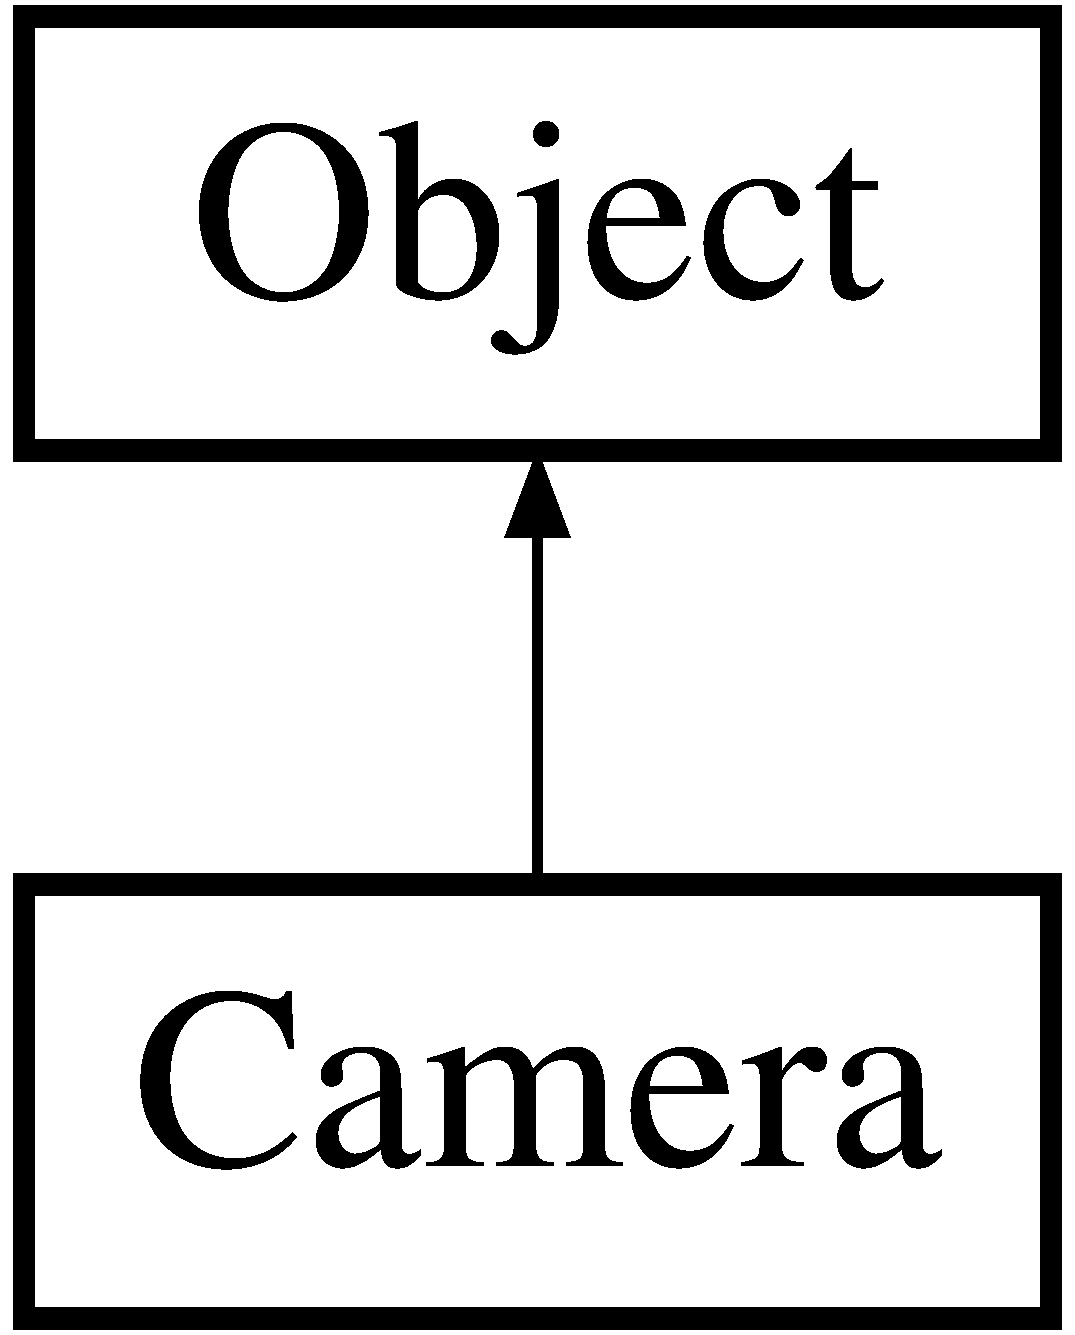
\includegraphics[height=2.000000cm]{class_camera}
\end{center}
\end{figure}
\subsection*{Public Member Functions}
\begin{DoxyCompactItemize}
\item 
\hyperlink{class_camera_a01f94c3543f56ede7af49dc778f19331}{Camera} ()
\begin{DoxyCompactList}\small\item\em Class constructor. \end{DoxyCompactList}\item 
\hyperlink{class_camera_ad1897942d0ccf91052386388a497349f}{$\sim$\+Camera} ()
\begin{DoxyCompactList}\small\item\em Class destructor. \end{DoxyCompactList}\item 
void \hyperlink{class_camera_ab8bb3c4e5dd304753fc6a2937175d1d9}{Set\+Persp\+Projection} (float fovy, float aspect, float near, float far)
\begin{DoxyCompactList}\small\item\em Perspective projection. \end{DoxyCompactList}\item 
void \hyperlink{class_camera_aaee3d9ca2a77a31574da1e927047af84}{Set\+Ortho\+Projection} (float left, float right, float bottom, float top, float near, float far)
\begin{DoxyCompactList}\small\item\em Orthographic projection. \end{DoxyCompactList}\item 
\hypertarget{class_camera_aaeadc93f9c5800d2b52af7f88c3ede5a}{}void {\bfseries Set\+View\+Matrix} (glm\+::mat4 view)\label{class_camera_aaeadc93f9c5800d2b52af7f88c3ede5a}

\item 
glm\+::mat4 $\ast$ \hyperlink{class_camera_a0a515e9b67a4f4f9d012209431e45448}{Get\+Projection} ()
\begin{DoxyCompactList}\small\item\em Returns the projection matrix. \end{DoxyCompactList}\item 
glm\+::mat4 $\ast$ \hyperlink{class_camera_a7a1951025a21533f97f06071df681f7b}{Get\+View} ()
\begin{DoxyCompactList}\small\item\em Returns the view matrix. \end{DoxyCompactList}\end{DoxyCompactItemize}
\subsection*{Additional Inherited Members}


\subsection{Detailed Description}
\hyperlink{class_camera}{Camera} class. 

Class used to control a camera. Contains essential functions like position, rotation and matrix projections 

\subsection{Constructor \& Destructor Documentation}
\hypertarget{class_camera_a01f94c3543f56ede7af49dc778f19331}{}\index{Camera@{Camera}!Camera@{Camera}}
\index{Camera@{Camera}!Camera@{Camera}}
\subsubsection[{Camera}]{\setlength{\rightskip}{0pt plus 5cm}Camera\+::\+Camera (
\begin{DoxyParamCaption}
{}
\end{DoxyParamCaption}
)}\label{class_camera_a01f94c3543f56ede7af49dc778f19331}


Class constructor. 

\hyperlink{class_camera}{Camera} class constructor. \hypertarget{class_camera_ad1897942d0ccf91052386388a497349f}{}\index{Camera@{Camera}!````~Camera@{$\sim$\+Camera}}
\index{````~Camera@{$\sim$\+Camera}!Camera@{Camera}}
\subsubsection[{$\sim$\+Camera}]{\setlength{\rightskip}{0pt plus 5cm}Camera\+::$\sim$\+Camera (
\begin{DoxyParamCaption}
{}
\end{DoxyParamCaption}
)}\label{class_camera_ad1897942d0ccf91052386388a497349f}


Class destructor. 

\hyperlink{class_camera}{Camera} class destructor. 

\subsection{Member Function Documentation}
\hypertarget{class_camera_a0a515e9b67a4f4f9d012209431e45448}{}\index{Camera@{Camera}!Get\+Projection@{Get\+Projection}}
\index{Get\+Projection@{Get\+Projection}!Camera@{Camera}}
\subsubsection[{Get\+Projection}]{\setlength{\rightskip}{0pt plus 5cm}glm\+::mat4 $\ast$ Camera\+::\+Get\+Projection (
\begin{DoxyParamCaption}
{}
\end{DoxyParamCaption}
)}\label{class_camera_a0a515e9b67a4f4f9d012209431e45448}


Returns the projection matrix. 

Returns the selected camera projection matrix (perspective or orthographic). \hypertarget{class_camera_a7a1951025a21533f97f06071df681f7b}{}\index{Camera@{Camera}!Get\+View@{Get\+View}}
\index{Get\+View@{Get\+View}!Camera@{Camera}}
\subsubsection[{Get\+View}]{\setlength{\rightskip}{0pt plus 5cm}glm\+::mat4 $\ast$ Camera\+::\+Get\+View (
\begin{DoxyParamCaption}
{}
\end{DoxyParamCaption}
)}\label{class_camera_a7a1951025a21533f97f06071df681f7b}


Returns the view matrix. 

Returns the camera view matrix. \hypertarget{class_camera_aaee3d9ca2a77a31574da1e927047af84}{}\index{Camera@{Camera}!Set\+Ortho\+Projection@{Set\+Ortho\+Projection}}
\index{Set\+Ortho\+Projection@{Set\+Ortho\+Projection}!Camera@{Camera}}
\subsubsection[{Set\+Ortho\+Projection}]{\setlength{\rightskip}{0pt plus 5cm}void Camera\+::\+Set\+Ortho\+Projection (
\begin{DoxyParamCaption}
\item[{float}]{left, }
\item[{float}]{right, }
\item[{float}]{bottom, }
\item[{float}]{top, }
\item[{float}]{near, }
\item[{float}]{far}
\end{DoxyParamCaption}
)}\label{class_camera_aaee3d9ca2a77a31574da1e927047af84}


Orthographic projection. 

Sets the camera with an orthographic projection matrix. 
\begin{DoxyParams}{Parameters}
{\em left} & Left camera frustum plane \\
\hline
{\em right} & Right camera frustum plane \\
\hline
{\em bottom} & Bottom camera frustum plane \\
\hline
{\em top} & Top camera frustum plane \\
\hline
{\em near} & Near plane \\
\hline
{\em far} & Far plane \\
\hline
\end{DoxyParams}
\hypertarget{class_camera_ab8bb3c4e5dd304753fc6a2937175d1d9}{}\index{Camera@{Camera}!Set\+Persp\+Projection@{Set\+Persp\+Projection}}
\index{Set\+Persp\+Projection@{Set\+Persp\+Projection}!Camera@{Camera}}
\subsubsection[{Set\+Persp\+Projection}]{\setlength{\rightskip}{0pt plus 5cm}void Camera\+::\+Set\+Persp\+Projection (
\begin{DoxyParamCaption}
\item[{float}]{fovy, }
\item[{float}]{aspect, }
\item[{float}]{near, }
\item[{float}]{far}
\end{DoxyParamCaption}
)}\label{class_camera_ab8bb3c4e5dd304753fc6a2937175d1d9}


Perspective projection. 

Sets the camera with a perspective projection matrix. 
\begin{DoxyParams}{Parameters}
{\em fovy} & Field of view \\
\hline
{\em aspect} & Aspect ratio \\
\hline
{\em near} & Near plane \\
\hline
{\em far} & Far plane \\
\hline
\end{DoxyParams}


The documentation for this class was generated from the following files\+:\begin{DoxyCompactItemize}
\item 
Camera.\+h\item 
Camera.\+cpp\end{DoxyCompactItemize}

\hypertarget{class_catmull_rom}{}\section{Catmull\+Rom Class Reference}
\label{class_catmull_rom}\index{Catmull\+Rom@{Catmull\+Rom}}
\subsection*{Public Member Functions}
\begin{DoxyCompactItemize}
\item 
\mbox{\Hypertarget{class_catmull_rom_a7c2ba84389cd456dd74cfc817fd6ae46}\label{class_catmull_rom_a7c2ba84389cd456dd74cfc817fd6ae46}} 
{\bfseries Catmull\+Rom} (glm\+::vec3 pointA, glm\+::vec3 pointB, glm\+::vec3 pointC, glm\+::vec3 pointD)
\item 
\mbox{\Hypertarget{class_catmull_rom_af77bf819993de8e541d3a7db5825faae}\label{class_catmull_rom_af77bf819993de8e541d3a7db5825faae}} 
glm\+::vec3 {\bfseries interpolate} (float t)
\end{DoxyCompactItemize}


The documentation for this class was generated from the following files\+:\begin{DoxyCompactItemize}
\item 
Catmull\+Rom.\+h\item 
Catmull\+Rom.\+cpp\end{DoxyCompactItemize}

\hypertarget{class_directional_light}{}\section{Directional\+Light Class Reference}
\label{class_directional_light}\index{Directional\+Light@{Directional\+Light}}


\hyperlink{class_directional_light}{Directional\+Light} class.  




{\ttfamily \#include $<$Directional\+Light.\+h$>$}

Inheritance diagram for Directional\+Light\+:\begin{figure}[H]
\begin{center}
\leavevmode
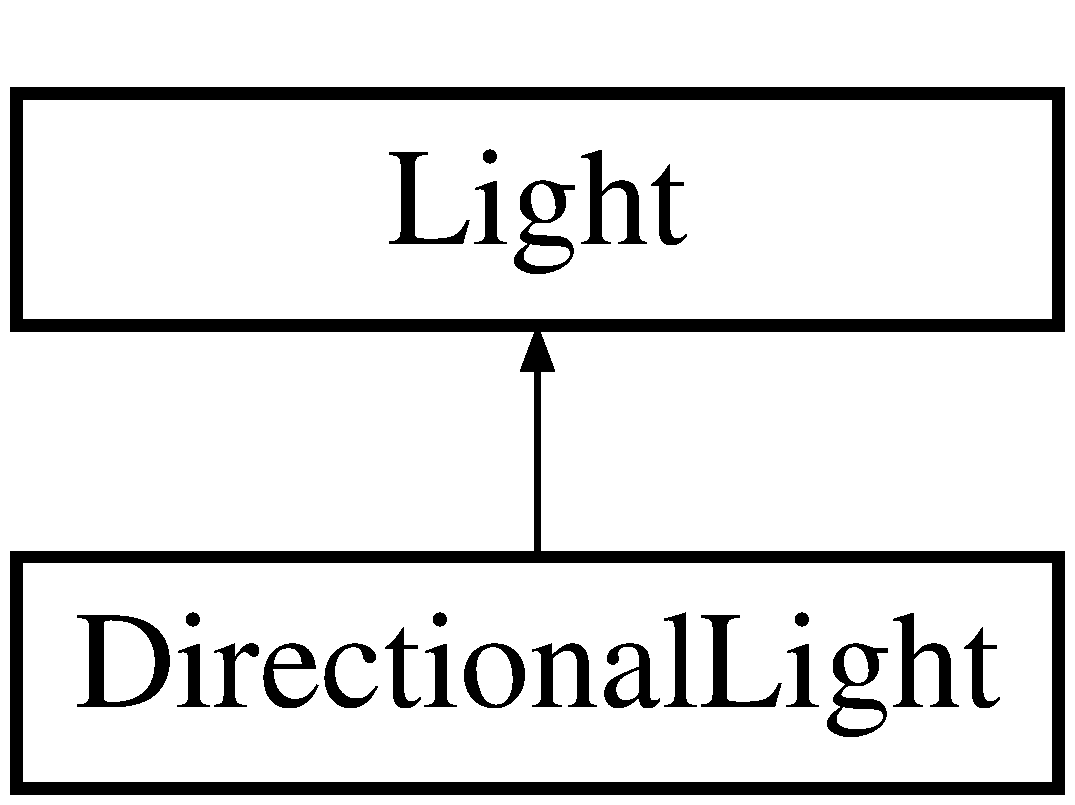
\includegraphics[height=2.000000cm]{class_directional_light}
\end{center}
\end{figure}
\subsection*{Public Member Functions}
\begin{DoxyCompactItemize}
\item 
\hyperlink{class_directional_light_a949b877ae041b9818f47eb812d80fa1b}{Directional\+Light} ()
\begin{DoxyCompactList}\small\item\em Class constructor. \end{DoxyCompactList}\item 
\hyperlink{class_directional_light_ac4aca6c806e752c65ffea9b2f237b245}{$\sim$\+Directional\+Light} ()
\begin{DoxyCompactList}\small\item\em Class destructor. \end{DoxyCompactList}\item 
void \hyperlink{class_directional_light_afdd5ff26965bdc32a0254af59332afd5}{Set\+Direction} (glm\+::vec3 position)
\begin{DoxyCompactList}\small\item\em Direction setter. \end{DoxyCompactList}\end{DoxyCompactItemize}
\subsection*{Additional Inherited Members}


\subsection{Detailed Description}
\hyperlink{class_directional_light}{Directional\+Light} class. 

Class used to define a directional light. 

\subsection{Constructor \& Destructor Documentation}
\mbox{\Hypertarget{class_directional_light_a949b877ae041b9818f47eb812d80fa1b}\label{class_directional_light_a949b877ae041b9818f47eb812d80fa1b}} 
\index{Directional\+Light@{Directional\+Light}!Directional\+Light@{Directional\+Light}}
\index{Directional\+Light@{Directional\+Light}!Directional\+Light@{Directional\+Light}}
\subsubsection{\texorpdfstring{Directional\+Light()}{DirectionalLight()}}
{\footnotesize\ttfamily Directional\+Light\+::\+Directional\+Light (\begin{DoxyParamCaption}{ }\end{DoxyParamCaption})}



Class constructor. 

\hyperlink{class_directional_light}{Directional\+Light} class constructor. \mbox{\Hypertarget{class_directional_light_ac4aca6c806e752c65ffea9b2f237b245}\label{class_directional_light_ac4aca6c806e752c65ffea9b2f237b245}} 
\index{Directional\+Light@{Directional\+Light}!````~Directional\+Light@{$\sim$\+Directional\+Light}}
\index{````~Directional\+Light@{$\sim$\+Directional\+Light}!Directional\+Light@{Directional\+Light}}
\subsubsection{\texorpdfstring{$\sim$\+Directional\+Light()}{~DirectionalLight()}}
{\footnotesize\ttfamily Directional\+Light\+::$\sim$\+Directional\+Light (\begin{DoxyParamCaption}{ }\end{DoxyParamCaption})}



Class destructor. 

\hyperlink{class_directional_light}{Directional\+Light} class destructor. 

\subsection{Member Function Documentation}
\mbox{\Hypertarget{class_directional_light_afdd5ff26965bdc32a0254af59332afd5}\label{class_directional_light_afdd5ff26965bdc32a0254af59332afd5}} 
\index{Directional\+Light@{Directional\+Light}!Set\+Direction@{Set\+Direction}}
\index{Set\+Direction@{Set\+Direction}!Directional\+Light@{Directional\+Light}}
\subsubsection{\texorpdfstring{Set\+Direction()}{SetDirection()}}
{\footnotesize\ttfamily void Directional\+Light\+::\+Set\+Direction (\begin{DoxyParamCaption}\item[{glm\+::vec3}]{position }\end{DoxyParamCaption})}



Direction setter. 


\begin{DoxyParams}{Parameters}
{\em direction} & 3D vector to set as new direction. \\
\hline
\end{DoxyParams}


The documentation for this class was generated from the following files\+:\begin{DoxyCompactItemize}
\item 
Directional\+Light.\+h\item 
Directional\+Light.\+cpp\end{DoxyCompactItemize}

\hypertarget{class_light}{}\section{Light Class Reference}
\label{class_light}\index{Light@{Light}}


\hyperlink{class_light}{Light} class.  




{\ttfamily \#include $<$Light.\+h$>$}

Inheritance diagram for Light\+:\begin{figure}[H]
\begin{center}
\leavevmode
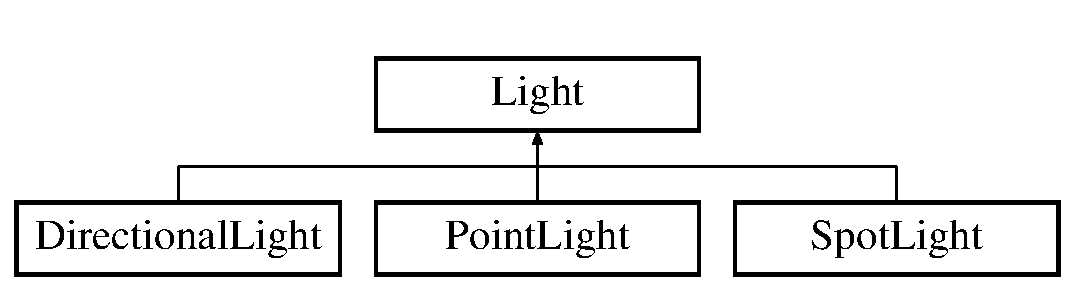
\includegraphics[height=2.000000cm]{class_light}
\end{center}
\end{figure}
\subsection*{Public Member Functions}
\begin{DoxyCompactItemize}
\item 
\hyperlink{class_light_aeb5df09a25a32f19fdffa761268ba24f}{Light} ()
\begin{DoxyCompactList}\small\item\em Class constructor. \end{DoxyCompactList}\item 
\hyperlink{class_light_ad0e59fad13bb6cfadc25b2c477e9ddc7}{$\sim$\+Light} ()
\begin{DoxyCompactList}\small\item\em Class destructor. \end{DoxyCompactList}\item 
glm\+::vec4 $\ast$ \hyperlink{class_light_a5ae42d0f1ff71f86b52ede3a37da455d}{Get\+Position} ()
\begin{DoxyCompactList}\small\item\em \hyperlink{class_light}{Light} position. \end{DoxyCompactList}\item 
glm\+::vec4 $\ast$ \hyperlink{class_light_a5373bb221bc648c203236d52b787416a}{Get\+Direction} ()
\begin{DoxyCompactList}\small\item\em \hyperlink{class_light}{Light} direction. \end{DoxyCompactList}\item 
glm\+::vec3 $\ast$ \hyperlink{class_light_ac017022a6e8dd3a29de1e024cfde9d9b}{Get\+Attenuation} ()
\begin{DoxyCompactList}\small\item\em \hyperlink{class_light}{Light} atternuation. \end{DoxyCompactList}\item 
G\+Lfloat \hyperlink{class_light_ad1ddee3ac2e66ee13e41544603587393}{Get\+Cos\+Cut\+Off} ()
\begin{DoxyCompactList}\small\item\em \hyperlink{class_light}{Light} cosine cut off. \end{DoxyCompactList}\item 
G\+Lfloat \hyperlink{class_light_ad40e4b5500b2b8d9be2ec76dc99e8868}{Get\+Spot\+Exponent} ()
\begin{DoxyCompactList}\small\item\em \hyperlink{class_light}{Light} spot exponent. \end{DoxyCompactList}\end{DoxyCompactItemize}
\subsection*{Public Attributes}
\begin{DoxyCompactItemize}
\item 
glm\+::vec3 \hyperlink{class_light_a3ddf6a283f42e3e3ce6a403b9477f7c2}{Ambient\+Color}
\begin{DoxyCompactList}\small\item\em Ambient color. \end{DoxyCompactList}\item 
glm\+::vec3 \hyperlink{class_light_ab3885005f09ec9411cc1f31c069dc7d9}{Diffuse\+Color}
\begin{DoxyCompactList}\small\item\em Diffuse color. \end{DoxyCompactList}\end{DoxyCompactItemize}
\subsection*{Protected Attributes}
\begin{DoxyCompactItemize}
\item 
glm\+::vec4 \hyperlink{class_light_a108cbac703d7fc2bc6eb39185d9bead9}{m\+\_\+pos}
\begin{DoxyCompactList}\small\item\em \hyperlink{class_light}{Light} postion. \end{DoxyCompactList}\item 
glm\+::vec4 \hyperlink{class_light_a837f0e73f495fd9361b6eecaafaef275}{m\+\_\+dir}
\begin{DoxyCompactList}\small\item\em \hyperlink{class_light}{Light} direction. \end{DoxyCompactList}\item 
glm\+::vec3 \hyperlink{class_light_a31a4d7e3042d7ffe99e3070bcaa6aa61}{m\+\_\+c}
\begin{DoxyCompactList}\small\item\em \hyperlink{class_light}{Light} attenuation. \end{DoxyCompactList}\item 
G\+Lfloat \hyperlink{class_light_a5f99e10dc1c5c49785c4523d09588eef}{m\+\_\+cos\+Cut\+Off}
\begin{DoxyCompactList}\small\item\em \hyperlink{class_light}{Light} cosine cut off. \end{DoxyCompactList}\item 
G\+Lfloat \hyperlink{class_light_a262000d67538f1a25613e18fe17668cd}{m\+\_\+spot\+Exponent}
\begin{DoxyCompactList}\small\item\em \hyperlink{class_light}{Light} spot exponent. \end{DoxyCompactList}\end{DoxyCompactItemize}


\subsection{Detailed Description}
\hyperlink{class_light}{Light} class. 

Base class for lights. All the lights must inherit from this class. 

\subsection{Constructor \& Destructor Documentation}
\mbox{\Hypertarget{class_light_aeb5df09a25a32f19fdffa761268ba24f}\label{class_light_aeb5df09a25a32f19fdffa761268ba24f}} 
\index{Light@{Light}!Light@{Light}}
\index{Light@{Light}!Light@{Light}}
\subsubsection{\texorpdfstring{Light()}{Light()}}
{\footnotesize\ttfamily Light\+::\+Light (\begin{DoxyParamCaption}{ }\end{DoxyParamCaption})}



Class constructor. 

\hyperlink{class_light}{Light} class constructor. \mbox{\Hypertarget{class_light_ad0e59fad13bb6cfadc25b2c477e9ddc7}\label{class_light_ad0e59fad13bb6cfadc25b2c477e9ddc7}} 
\index{Light@{Light}!````~Light@{$\sim$\+Light}}
\index{````~Light@{$\sim$\+Light}!Light@{Light}}
\subsubsection{\texorpdfstring{$\sim$\+Light()}{~Light()}}
{\footnotesize\ttfamily Light\+::$\sim$\+Light (\begin{DoxyParamCaption}{ }\end{DoxyParamCaption})}



Class destructor. 

\hyperlink{class_light}{Light} class destructor. 

\subsection{Member Function Documentation}
\mbox{\Hypertarget{class_light_ac017022a6e8dd3a29de1e024cfde9d9b}\label{class_light_ac017022a6e8dd3a29de1e024cfde9d9b}} 
\index{Light@{Light}!Get\+Attenuation@{Get\+Attenuation}}
\index{Get\+Attenuation@{Get\+Attenuation}!Light@{Light}}
\subsubsection{\texorpdfstring{Get\+Attenuation()}{GetAttenuation()}}
{\footnotesize\ttfamily glm\+::vec3 $\ast$ Light\+::\+Get\+Attenuation (\begin{DoxyParamCaption}{ }\end{DoxyParamCaption})}



\hyperlink{class_light}{Light} atternuation. 

Returns the atternuation of the light. \mbox{\Hypertarget{class_light_ad1ddee3ac2e66ee13e41544603587393}\label{class_light_ad1ddee3ac2e66ee13e41544603587393}} 
\index{Light@{Light}!Get\+Cos\+Cut\+Off@{Get\+Cos\+Cut\+Off}}
\index{Get\+Cos\+Cut\+Off@{Get\+Cos\+Cut\+Off}!Light@{Light}}
\subsubsection{\texorpdfstring{Get\+Cos\+Cut\+Off()}{GetCosCutOff()}}
{\footnotesize\ttfamily G\+Lfloat Light\+::\+Get\+Cos\+Cut\+Off (\begin{DoxyParamCaption}{ }\end{DoxyParamCaption})}



\hyperlink{class_light}{Light} cosine cut off. 

Returns the cosine of the cut off of the light. If it is a directional or a spot light returns -\/1. \mbox{\Hypertarget{class_light_a5373bb221bc648c203236d52b787416a}\label{class_light_a5373bb221bc648c203236d52b787416a}} 
\index{Light@{Light}!Get\+Direction@{Get\+Direction}}
\index{Get\+Direction@{Get\+Direction}!Light@{Light}}
\subsubsection{\texorpdfstring{Get\+Direction()}{GetDirection()}}
{\footnotesize\ttfamily glm\+::vec4 $\ast$ Light\+::\+Get\+Direction (\begin{DoxyParamCaption}{ }\end{DoxyParamCaption})}



\hyperlink{class_light}{Light} direction. 

Returns the direction of the light. \mbox{\Hypertarget{class_light_a5ae42d0f1ff71f86b52ede3a37da455d}\label{class_light_a5ae42d0f1ff71f86b52ede3a37da455d}} 
\index{Light@{Light}!Get\+Position@{Get\+Position}}
\index{Get\+Position@{Get\+Position}!Light@{Light}}
\subsubsection{\texorpdfstring{Get\+Position()}{GetPosition()}}
{\footnotesize\ttfamily glm\+::vec4 $\ast$ Light\+::\+Get\+Position (\begin{DoxyParamCaption}{ }\end{DoxyParamCaption})}



\hyperlink{class_light}{Light} position. 

Returns the position of the light. \mbox{\Hypertarget{class_light_ad40e4b5500b2b8d9be2ec76dc99e8868}\label{class_light_ad40e4b5500b2b8d9be2ec76dc99e8868}} 
\index{Light@{Light}!Get\+Spot\+Exponent@{Get\+Spot\+Exponent}}
\index{Get\+Spot\+Exponent@{Get\+Spot\+Exponent}!Light@{Light}}
\subsubsection{\texorpdfstring{Get\+Spot\+Exponent()}{GetSpotExponent()}}
{\footnotesize\ttfamily G\+Lfloat Light\+::\+Get\+Spot\+Exponent (\begin{DoxyParamCaption}{ }\end{DoxyParamCaption})}



\hyperlink{class_light}{Light} spot exponent. 

Returns the spot exponent of the light. If it is a directional or a spot light returns 0. 

\subsection{Member Data Documentation}
\mbox{\Hypertarget{class_light_a3ddf6a283f42e3e3ce6a403b9477f7c2}\label{class_light_a3ddf6a283f42e3e3ce6a403b9477f7c2}} 
\index{Light@{Light}!Ambient\+Color@{Ambient\+Color}}
\index{Ambient\+Color@{Ambient\+Color}!Light@{Light}}
\subsubsection{\texorpdfstring{Ambient\+Color}{AmbientColor}}
{\footnotesize\ttfamily glm\+::vec3 Light\+::\+Ambient\+Color}



Ambient color. 

Ambient color of the light. \mbox{\Hypertarget{class_light_ab3885005f09ec9411cc1f31c069dc7d9}\label{class_light_ab3885005f09ec9411cc1f31c069dc7d9}} 
\index{Light@{Light}!Diffuse\+Color@{Diffuse\+Color}}
\index{Diffuse\+Color@{Diffuse\+Color}!Light@{Light}}
\subsubsection{\texorpdfstring{Diffuse\+Color}{DiffuseColor}}
{\footnotesize\ttfamily glm\+::vec3 Light\+::\+Diffuse\+Color}



Diffuse color. 

Diffuse color of the light. \mbox{\Hypertarget{class_light_a31a4d7e3042d7ffe99e3070bcaa6aa61}\label{class_light_a31a4d7e3042d7ffe99e3070bcaa6aa61}} 
\index{Light@{Light}!m\+\_\+c@{m\+\_\+c}}
\index{m\+\_\+c@{m\+\_\+c}!Light@{Light}}
\subsubsection{\texorpdfstring{m\+\_\+c}{m\_c}}
{\footnotesize\ttfamily glm\+::vec3 Light\+::m\+\_\+c\hspace{0.3cm}{\ttfamily [protected]}}



\hyperlink{class_light}{Light} attenuation. 

\hyperlink{class_light}{Light} attenuation. \mbox{\Hypertarget{class_light_a5f99e10dc1c5c49785c4523d09588eef}\label{class_light_a5f99e10dc1c5c49785c4523d09588eef}} 
\index{Light@{Light}!m\+\_\+cos\+Cut\+Off@{m\+\_\+cos\+Cut\+Off}}
\index{m\+\_\+cos\+Cut\+Off@{m\+\_\+cos\+Cut\+Off}!Light@{Light}}
\subsubsection{\texorpdfstring{m\+\_\+cos\+Cut\+Off}{m\_cosCutOff}}
{\footnotesize\ttfamily G\+Lfloat Light\+::m\+\_\+cos\+Cut\+Off\hspace{0.3cm}{\ttfamily [protected]}}



\hyperlink{class_light}{Light} cosine cut off. 

\hyperlink{class_light}{Light} cosine cut off. \mbox{\Hypertarget{class_light_a837f0e73f495fd9361b6eecaafaef275}\label{class_light_a837f0e73f495fd9361b6eecaafaef275}} 
\index{Light@{Light}!m\+\_\+dir@{m\+\_\+dir}}
\index{m\+\_\+dir@{m\+\_\+dir}!Light@{Light}}
\subsubsection{\texorpdfstring{m\+\_\+dir}{m\_dir}}
{\footnotesize\ttfamily glm\+::vec4 Light\+::m\+\_\+dir\hspace{0.3cm}{\ttfamily [protected]}}



\hyperlink{class_light}{Light} direction. 

\hyperlink{class_light}{Light} direction. \mbox{\Hypertarget{class_light_a108cbac703d7fc2bc6eb39185d9bead9}\label{class_light_a108cbac703d7fc2bc6eb39185d9bead9}} 
\index{Light@{Light}!m\+\_\+pos@{m\+\_\+pos}}
\index{m\+\_\+pos@{m\+\_\+pos}!Light@{Light}}
\subsubsection{\texorpdfstring{m\+\_\+pos}{m\_pos}}
{\footnotesize\ttfamily glm\+::vec4 Light\+::m\+\_\+pos\hspace{0.3cm}{\ttfamily [protected]}}



\hyperlink{class_light}{Light} postion. 

\hyperlink{class_light}{Light} position. \mbox{\Hypertarget{class_light_a262000d67538f1a25613e18fe17668cd}\label{class_light_a262000d67538f1a25613e18fe17668cd}} 
\index{Light@{Light}!m\+\_\+spot\+Exponent@{m\+\_\+spot\+Exponent}}
\index{m\+\_\+spot\+Exponent@{m\+\_\+spot\+Exponent}!Light@{Light}}
\subsubsection{\texorpdfstring{m\+\_\+spot\+Exponent}{m\_spotExponent}}
{\footnotesize\ttfamily G\+Lfloat Light\+::m\+\_\+spot\+Exponent\hspace{0.3cm}{\ttfamily [protected]}}



\hyperlink{class_light}{Light} spot exponent. 

\hyperlink{class_light}{Light} spot exponent. 

The documentation for this class was generated from the following files\+:\begin{DoxyCompactItemize}
\item 
Light.\+h\item 
Light.\+cpp\end{DoxyCompactItemize}

\hypertarget{struct_light_params}{}\section{Light\+Params Struct Reference}
\label{struct_light_params}\index{Light\+Params@{Light\+Params}}
\subsection*{Public Attributes}
\begin{DoxyCompactItemize}
\item 
\hypertarget{struct_light_params_ad7ba6aa7e333ba4552cddce6e58ee11b}{}int {\bfseries u\+Amb}\label{struct_light_params_ad7ba6aa7e333ba4552cddce6e58ee11b}

\item 
\hypertarget{struct_light_params_a4b08902022f1049975054635ab02a373}{}int {\bfseries u\+Diff}\label{struct_light_params_a4b08902022f1049975054635ab02a373}

\item 
\hypertarget{struct_light_params_af93dcacd5dc9afa86f47c1fc6dafd1de}{}int {\bfseries u\+Pos}\label{struct_light_params_af93dcacd5dc9afa86f47c1fc6dafd1de}

\item 
\hypertarget{struct_light_params_a2c5ef6397619c3d9f9ebc3f85a60e271}{}int {\bfseries u\+Dir}\label{struct_light_params_a2c5ef6397619c3d9f9ebc3f85a60e271}

\item 
\hypertarget{struct_light_params_a19c2f90d8bd6212458a36faba22a25d3}{}int {\bfseries u\+C}\label{struct_light_params_a19c2f90d8bd6212458a36faba22a25d3}

\item 
\hypertarget{struct_light_params_aede0ecb733b98b5d9fa9aea079a19e32}{}int {\bfseries u\+Cos\+Cut\+Off}\label{struct_light_params_aede0ecb733b98b5d9fa9aea079a19e32}

\item 
\hypertarget{struct_light_params_af5f5bd61015288e5fe8c4fe99ae22948}{}int {\bfseries u\+Spot\+Exponent}\label{struct_light_params_af5f5bd61015288e5fe8c4fe99ae22948}

\item 
\hypertarget{struct_light_params_a27052b5211820c45d996f5106880514d}{}glm\+::vec3 {\bfseries Amb}\label{struct_light_params_a27052b5211820c45d996f5106880514d}

\item 
\hypertarget{struct_light_params_a68f0078bf3744578ae5a655365c913b1}{}glm\+::vec3 {\bfseries Diff}\label{struct_light_params_a68f0078bf3744578ae5a655365c913b1}

\item 
\hypertarget{struct_light_params_ad7dd75d1bf55dd855ced7c5cd48a0a94}{}glm\+::vec4 {\bfseries Pos}\label{struct_light_params_ad7dd75d1bf55dd855ced7c5cd48a0a94}

\item 
\hypertarget{struct_light_params_af3eff9a35c7e1d5606a82bccc1bfeeec}{}glm\+::vec4 {\bfseries Dir}\label{struct_light_params_af3eff9a35c7e1d5606a82bccc1bfeeec}

\item 
\hypertarget{struct_light_params_ab5f4306c4f1c855a4b34b55a91efc8cf}{}glm\+::vec3 {\bfseries C}\label{struct_light_params_ab5f4306c4f1c855a4b34b55a91efc8cf}

\item 
\hypertarget{struct_light_params_aff1247010ed10eb06ff787bfc275dc4b}{}G\+Lfloat {\bfseries Cos\+Cut\+Off}\label{struct_light_params_aff1247010ed10eb06ff787bfc275dc4b}

\item 
\hypertarget{struct_light_params_a29a0354e2f5b4571b6ced4ff281e53c8}{}G\+Lfloat {\bfseries Spot\+Exponent}\label{struct_light_params_a29a0354e2f5b4571b6ced4ff281e53c8}

\end{DoxyCompactItemize}


The documentation for this struct was generated from the following file\+:\begin{DoxyCompactItemize}
\item 
main.\+cpp\end{DoxyCompactItemize}

\hypertarget{class_mesh}{}\section{Mesh Class Reference}
\label{class_mesh}\index{Mesh@{Mesh}}


\hyperlink{class_mesh}{Mesh} class.  




{\ttfamily \#include $<$Mesh.\+h$>$}

\subsection*{Public Member Functions}
\begin{DoxyCompactItemize}
\item 
\hyperlink{class_mesh_a7cb142bf7cd75a954813ccebe1780b77}{Mesh} (const char $\ast$file, \hyperlink{class_shader}{Shader} $\ast$material)
\begin{DoxyCompactList}\small\item\em Class constructor. \end{DoxyCompactList}\item 
\hyperlink{class_mesh_a6b89dd43d75a4c8d5597f88cf7645488}{Mesh} (const unsigned int n\+Triangles, const unsigned int n\+Vertex, const unsigned int $\ast$index, const float $\ast$pos, \hyperlink{class_shader}{Shader} $\ast$material, const float $\ast$n=nullptr, const float $\ast$color=nullptr, const float $\ast$tex=nullptr, const float $\ast$tangent=nullptr)
\begin{DoxyCompactList}\small\item\em Class constructor. \end{DoxyCompactList}\item 
void \hyperlink{class_mesh_a0cf8b6c8062509bd89d8bcc773f45c64}{Apply\+Material} (\hyperlink{class_shader}{Shader} $\ast$material)
\begin{DoxyCompactList}\small\item\em Function to set a shader in charge of render this mesh. \end{DoxyCompactList}\item 
unsigned int $\ast$ \hyperlink{class_mesh_a99962ed2f4a6a0999127f5e4defef6dc}{get\+Triangle\+Index} ()
\begin{DoxyCompactList}\small\item\em Triangles index getter. \end{DoxyCompactList}\item 
float $\ast$ \hyperlink{class_mesh_a2345e6c20aa6a0f05521b8aeb62203f4}{get\+Vertex\+Pos} ()
\begin{DoxyCompactList}\small\item\em Vertices position getter. \end{DoxyCompactList}\item 
float $\ast$ \hyperlink{class_mesh_ab16f1115ed7865c9e7322c85e2d785af}{get\+Vertex\+Normals} ()
\begin{DoxyCompactList}\small\item\em Vertices normal getter. \end{DoxyCompactList}\item 
float $\ast$ \hyperlink{class_mesh_ade2dd22f7cbe37df8e51ba65c800bbc8}{get\+Vertex\+Color} ()
\begin{DoxyCompactList}\small\item\em Vertices color getter. \end{DoxyCompactList}\item 
float $\ast$ \hyperlink{class_mesh_ab6ba57a10fbed17d8f9dc8ec09b92657}{get\+Vertex\+Tex\+Coord} ()
\begin{DoxyCompactList}\small\item\em Vertices texture coordinates getter. \end{DoxyCompactList}\item 
float $\ast$ \hyperlink{class_mesh_ae5cd8d05ef13c4e71bea276a9783adaf}{get\+Vertex\+Tangent} ()
\begin{DoxyCompactList}\small\item\em Vertices tangent getter. \end{DoxyCompactList}\item 
unsigned int \hyperlink{class_mesh_a838bd5498ec781707bb28830ff5e064d}{get\+Color\+Tex} ()
\begin{DoxyCompactList}\small\item\em Color texture getter. \end{DoxyCompactList}\item 
unsigned int \hyperlink{class_mesh_ad4787ea15b5ad63eed00a1a0ef272637}{get\+Spec\+Tex} ()
\begin{DoxyCompactList}\small\item\em Specular texture getter. \end{DoxyCompactList}\item 
unsigned int \hyperlink{class_mesh_ad0b8c57f20a5319e2e730cfa61271904}{get\+Emi\+Tex} ()
\begin{DoxyCompactList}\small\item\em Emissive texture getter. \end{DoxyCompactList}\item 
unsigned int \hyperlink{class_mesh_a8b60518f329c4e3d15824ef68c794fa1}{get\+Norm\+Tex} ()
\begin{DoxyCompactList}\small\item\em Normal texture getter. \end{DoxyCompactList}\item 
unsigned int \hyperlink{class_mesh_add2e2bafe60711ec9f67308c140640a9}{get\+V\+AO} ()
\begin{DoxyCompactList}\small\item\em V\+AO ID getter. \end{DoxyCompactList}\item 
int \hyperlink{class_mesh_ae4163571bceed9d224fc43e943dda118}{get\+Num\+Vertex} ()
\begin{DoxyCompactList}\small\item\em Number of vertex getter. \end{DoxyCompactList}\item 
int \hyperlink{class_mesh_a4452aed4ac63ff0639b839bba095347e}{get\+Num\+Triangles} ()
\begin{DoxyCompactList}\small\item\em Number of triangles. \end{DoxyCompactList}\item 
bool \hyperlink{class_mesh_ac06b928f547c1eec3b66ae5503608c21}{load\+Color\+Tex} (const char $\ast$file)
\begin{DoxyCompactList}\small\item\em Color texture loader. \end{DoxyCompactList}\item 
bool \hyperlink{class_mesh_ada437d0826057661de46ab5ce2b497a4}{load\+Spec\+Tex} (const char $\ast$file)
\begin{DoxyCompactList}\small\item\em Specular texture loader. \end{DoxyCompactList}\item 
bool \hyperlink{class_mesh_abb21ce55711b89f7018d103b50294f69}{load\+Emi\+Tex} (const char $\ast$file)
\begin{DoxyCompactList}\small\item\em Emissive texture loader. \end{DoxyCompactList}\item 
bool \hyperlink{class_mesh_a443b1a0a0c36ff911f58f2a5f4616538}{load\+Norm\+Tex} (const char $\ast$file)
\begin{DoxyCompactList}\small\item\em Normal texture loader. \end{DoxyCompactList}\item 
void \hyperlink{class_mesh_a81e2edec37429d2830a551d07476c7ba}{add\+Object} (\hyperlink{class_object}{Object} $\ast$o)
\begin{DoxyCompactList}\small\item\em Function to add object so they use this mesh. \end{DoxyCompactList}\item 
void \hyperlink{class_mesh_a7c209ba6e5596edaeb9062cf23d3532b}{remove\+Object} (\hyperlink{class_object}{Object} $\ast$o)
\begin{DoxyCompactList}\small\item\em Function to remove using this mesh. \end{DoxyCompactList}\item 
std\+::list$<$ \hyperlink{class_object}{Object} $\ast$ $>$ \& \hyperlink{class_mesh_aadc3cc59b0dccf99961105431a717579}{get\+Objects} ()
\begin{DoxyCompactList}\small\item\em Function to obtain the list of Objects using this mesh. \end{DoxyCompactList}\item 
\hyperlink{class_mesh_a5efe4da1a4c0971cfb037bd70304c303}{$\sim$\+Mesh} ()
\begin{DoxyCompactList}\small\item\em \hyperlink{class_mesh}{Mesh} class destructor. \end{DoxyCompactList}\end{DoxyCompactItemize}


\subsection{Detailed Description}
\hyperlink{class_mesh}{Mesh} class. 

Class used to define and control a mesh. Contains functions related with its points, textures and properties. 

\subsection{Constructor \& Destructor Documentation}
\mbox{\Hypertarget{class_mesh_a7cb142bf7cd75a954813ccebe1780b77}\label{class_mesh_a7cb142bf7cd75a954813ccebe1780b77}} 
\index{Mesh@{Mesh}!Mesh@{Mesh}}
\index{Mesh@{Mesh}!Mesh@{Mesh}}
\subsubsection{\texorpdfstring{Mesh()}{Mesh()}\hspace{0.1cm}{\footnotesize\ttfamily [1/2]}}
{\footnotesize\ttfamily Mesh\+::\+Mesh (\begin{DoxyParamCaption}\item[{const char $\ast$}]{file,  }\item[{\hyperlink{class_shader}{Shader} $\ast$}]{material }\end{DoxyParamCaption})}



Class constructor. 

\hyperlink{class_mesh}{Mesh} class constructor.


\begin{DoxyParams}{Parameters}
{\em file} & File where the mesh is stored. \\
\hline
{\em material} & \hyperlink{class_shader}{Shader} that will render the mesh. \\
\hline
\end{DoxyParams}
\mbox{\Hypertarget{class_mesh_a6b89dd43d75a4c8d5597f88cf7645488}\label{class_mesh_a6b89dd43d75a4c8d5597f88cf7645488}} 
\index{Mesh@{Mesh}!Mesh@{Mesh}}
\index{Mesh@{Mesh}!Mesh@{Mesh}}
\subsubsection{\texorpdfstring{Mesh()}{Mesh()}\hspace{0.1cm}{\footnotesize\ttfamily [2/2]}}
{\footnotesize\ttfamily Mesh\+::\+Mesh (\begin{DoxyParamCaption}\item[{const unsigned int}]{n\+Triangles,  }\item[{const unsigned int}]{n\+Vertex,  }\item[{const unsigned int $\ast$}]{index,  }\item[{const float $\ast$}]{pos,  }\item[{\hyperlink{class_shader}{Shader} $\ast$}]{material,  }\item[{const float $\ast$}]{n = {\ttfamily nullptr},  }\item[{const float $\ast$}]{color = {\ttfamily nullptr},  }\item[{const float $\ast$}]{tex = {\ttfamily nullptr},  }\item[{const float $\ast$}]{tangent = {\ttfamily nullptr} }\end{DoxyParamCaption})}



Class constructor. 

\hyperlink{class_mesh}{Mesh} class constructor.


\begin{DoxyParams}{Parameters}
{\em n\+Triangles} & Number of triangles in the mesh. \\
\hline
{\em n\+Vertex} & Number of vertex in the mesh. \\
\hline
{\em index} & Array of vertex index. \\
\hline
{\em pos} & Array of vertex positions. \\
\hline
{\em material} & \hyperlink{class_shader}{Shader} that will render the mesh. \\
\hline
{\em n} & Array of vertex normals. \\
\hline
{\em tex} & Array of vertex texture coordinates. \\
\hline
{\em tangent} & Array of vertex tangents. \\
\hline
\end{DoxyParams}
\mbox{\Hypertarget{class_mesh_a5efe4da1a4c0971cfb037bd70304c303}\label{class_mesh_a5efe4da1a4c0971cfb037bd70304c303}} 
\index{Mesh@{Mesh}!````~Mesh@{$\sim$\+Mesh}}
\index{````~Mesh@{$\sim$\+Mesh}!Mesh@{Mesh}}
\subsubsection{\texorpdfstring{$\sim$\+Mesh()}{~Mesh()}}
{\footnotesize\ttfamily Mesh\+::$\sim$\+Mesh (\begin{DoxyParamCaption}{ }\end{DoxyParamCaption})}



\hyperlink{class_mesh}{Mesh} class destructor. 

Frees all memory used by all the textures and buffers in this mesh. 

\subsection{Member Function Documentation}
\mbox{\Hypertarget{class_mesh_a81e2edec37429d2830a551d07476c7ba}\label{class_mesh_a81e2edec37429d2830a551d07476c7ba}} 
\index{Mesh@{Mesh}!add\+Object@{add\+Object}}
\index{add\+Object@{add\+Object}!Mesh@{Mesh}}
\subsubsection{\texorpdfstring{add\+Object()}{addObject()}}
{\footnotesize\ttfamily void Mesh\+::add\+Object (\begin{DoxyParamCaption}\item[{\hyperlink{class_object}{Object} $\ast$}]{o }\end{DoxyParamCaption})}



Function to add object so they use this mesh. 


\begin{DoxyParams}{Parameters}
{\em o} & \hyperlink{class_object}{Object} to add. Sets a object to use this mesh. \\
\hline
\end{DoxyParams}
\mbox{\Hypertarget{class_mesh_a0cf8b6c8062509bd89d8bcc773f45c64}\label{class_mesh_a0cf8b6c8062509bd89d8bcc773f45c64}} 
\index{Mesh@{Mesh}!Apply\+Material@{Apply\+Material}}
\index{Apply\+Material@{Apply\+Material}!Mesh@{Mesh}}
\subsubsection{\texorpdfstring{Apply\+Material()}{ApplyMaterial()}}
{\footnotesize\ttfamily void Mesh\+::\+Apply\+Material (\begin{DoxyParamCaption}\item[{\hyperlink{class_shader}{Shader} $\ast$}]{material }\end{DoxyParamCaption})}



Function to set a shader in charge of render this mesh. 

Sets the shader used to render this mesh.


\begin{DoxyParams}{Parameters}
{\em material} & \hyperlink{class_shader}{Shader} to use. \\
\hline
\end{DoxyParams}
\mbox{\Hypertarget{class_mesh_a838bd5498ec781707bb28830ff5e064d}\label{class_mesh_a838bd5498ec781707bb28830ff5e064d}} 
\index{Mesh@{Mesh}!get\+Color\+Tex@{get\+Color\+Tex}}
\index{get\+Color\+Tex@{get\+Color\+Tex}!Mesh@{Mesh}}
\subsubsection{\texorpdfstring{get\+Color\+Tex()}{getColorTex()}}
{\footnotesize\ttfamily unsigned int Mesh\+::get\+Color\+Tex (\begin{DoxyParamCaption}{ }\end{DoxyParamCaption})}



Color texture getter. 

\begin{DoxyReturn}{Returns}
The color texture ID. 
\end{DoxyReturn}
\mbox{\Hypertarget{class_mesh_ad0b8c57f20a5319e2e730cfa61271904}\label{class_mesh_ad0b8c57f20a5319e2e730cfa61271904}} 
\index{Mesh@{Mesh}!get\+Emi\+Tex@{get\+Emi\+Tex}}
\index{get\+Emi\+Tex@{get\+Emi\+Tex}!Mesh@{Mesh}}
\subsubsection{\texorpdfstring{get\+Emi\+Tex()}{getEmiTex()}}
{\footnotesize\ttfamily unsigned int Mesh\+::get\+Emi\+Tex (\begin{DoxyParamCaption}{ }\end{DoxyParamCaption})}



Emissive texture getter. 

\begin{DoxyReturn}{Returns}
The emissive texture ID. 
\end{DoxyReturn}
\mbox{\Hypertarget{class_mesh_a8b60518f329c4e3d15824ef68c794fa1}\label{class_mesh_a8b60518f329c4e3d15824ef68c794fa1}} 
\index{Mesh@{Mesh}!get\+Norm\+Tex@{get\+Norm\+Tex}}
\index{get\+Norm\+Tex@{get\+Norm\+Tex}!Mesh@{Mesh}}
\subsubsection{\texorpdfstring{get\+Norm\+Tex()}{getNormTex()}}
{\footnotesize\ttfamily unsigned int Mesh\+::get\+Norm\+Tex (\begin{DoxyParamCaption}{ }\end{DoxyParamCaption})}



Normal texture getter. 

\begin{DoxyReturn}{Returns}
The normal texture ID. 
\end{DoxyReturn}
\mbox{\Hypertarget{class_mesh_a4452aed4ac63ff0639b839bba095347e}\label{class_mesh_a4452aed4ac63ff0639b839bba095347e}} 
\index{Mesh@{Mesh}!get\+Num\+Triangles@{get\+Num\+Triangles}}
\index{get\+Num\+Triangles@{get\+Num\+Triangles}!Mesh@{Mesh}}
\subsubsection{\texorpdfstring{get\+Num\+Triangles()}{getNumTriangles()}}
{\footnotesize\ttfamily int Mesh\+::get\+Num\+Triangles (\begin{DoxyParamCaption}{ }\end{DoxyParamCaption})}



Number of triangles. 

\begin{DoxyReturn}{Returns}
The number of triangles in the mesh. 
\end{DoxyReturn}
\mbox{\Hypertarget{class_mesh_ae4163571bceed9d224fc43e943dda118}\label{class_mesh_ae4163571bceed9d224fc43e943dda118}} 
\index{Mesh@{Mesh}!get\+Num\+Vertex@{get\+Num\+Vertex}}
\index{get\+Num\+Vertex@{get\+Num\+Vertex}!Mesh@{Mesh}}
\subsubsection{\texorpdfstring{get\+Num\+Vertex()}{getNumVertex()}}
{\footnotesize\ttfamily int Mesh\+::get\+Num\+Vertex (\begin{DoxyParamCaption}{ }\end{DoxyParamCaption})}



Number of vertex getter. 

\begin{DoxyReturn}{Returns}
The number of vertex in the mesh. 
\end{DoxyReturn}
\mbox{\Hypertarget{class_mesh_aadc3cc59b0dccf99961105431a717579}\label{class_mesh_aadc3cc59b0dccf99961105431a717579}} 
\index{Mesh@{Mesh}!get\+Objects@{get\+Objects}}
\index{get\+Objects@{get\+Objects}!Mesh@{Mesh}}
\subsubsection{\texorpdfstring{get\+Objects()}{getObjects()}}
{\footnotesize\ttfamily std\+::list$<$ \hyperlink{class_object}{Object} $\ast$ $>$ \& Mesh\+::get\+Objects (\begin{DoxyParamCaption}{ }\end{DoxyParamCaption})}



Function to obtain the list of Objects using this mesh. 

\begin{DoxyReturn}{Returns}
A list with pointers to all objects using this mesh. 
\end{DoxyReturn}
\mbox{\Hypertarget{class_mesh_ad4787ea15b5ad63eed00a1a0ef272637}\label{class_mesh_ad4787ea15b5ad63eed00a1a0ef272637}} 
\index{Mesh@{Mesh}!get\+Spec\+Tex@{get\+Spec\+Tex}}
\index{get\+Spec\+Tex@{get\+Spec\+Tex}!Mesh@{Mesh}}
\subsubsection{\texorpdfstring{get\+Spec\+Tex()}{getSpecTex()}}
{\footnotesize\ttfamily unsigned int Mesh\+::get\+Spec\+Tex (\begin{DoxyParamCaption}{ }\end{DoxyParamCaption})}



Specular texture getter. 

\begin{DoxyReturn}{Returns}
The specular texture ID. 
\end{DoxyReturn}
\mbox{\Hypertarget{class_mesh_a99962ed2f4a6a0999127f5e4defef6dc}\label{class_mesh_a99962ed2f4a6a0999127f5e4defef6dc}} 
\index{Mesh@{Mesh}!get\+Triangle\+Index@{get\+Triangle\+Index}}
\index{get\+Triangle\+Index@{get\+Triangle\+Index}!Mesh@{Mesh}}
\subsubsection{\texorpdfstring{get\+Triangle\+Index()}{getTriangleIndex()}}
{\footnotesize\ttfamily unsigned int $\ast$ Mesh\+::get\+Triangle\+Index (\begin{DoxyParamCaption}{ }\end{DoxyParamCaption})}



Triangles index getter. 

\begin{DoxyReturn}{Returns}
A pointer to the triangles index array. 
\end{DoxyReturn}
\mbox{\Hypertarget{class_mesh_add2e2bafe60711ec9f67308c140640a9}\label{class_mesh_add2e2bafe60711ec9f67308c140640a9}} 
\index{Mesh@{Mesh}!get\+V\+AO@{get\+V\+AO}}
\index{get\+V\+AO@{get\+V\+AO}!Mesh@{Mesh}}
\subsubsection{\texorpdfstring{get\+V\+A\+O()}{getVAO()}}
{\footnotesize\ttfamily unsigned int Mesh\+::get\+V\+AO (\begin{DoxyParamCaption}{ }\end{DoxyParamCaption})}



V\+AO ID getter. 

\begin{DoxyReturn}{Returns}
V\+AO ID. 
\end{DoxyReturn}
\mbox{\Hypertarget{class_mesh_ade2dd22f7cbe37df8e51ba65c800bbc8}\label{class_mesh_ade2dd22f7cbe37df8e51ba65c800bbc8}} 
\index{Mesh@{Mesh}!get\+Vertex\+Color@{get\+Vertex\+Color}}
\index{get\+Vertex\+Color@{get\+Vertex\+Color}!Mesh@{Mesh}}
\subsubsection{\texorpdfstring{get\+Vertex\+Color()}{getVertexColor()}}
{\footnotesize\ttfamily float $\ast$ Mesh\+::get\+Vertex\+Color (\begin{DoxyParamCaption}{ }\end{DoxyParamCaption})}



Vertices color getter. 

\begin{DoxyReturn}{Returns}
A pointer to the vertices normal array. 
\end{DoxyReturn}
\mbox{\Hypertarget{class_mesh_ab16f1115ed7865c9e7322c85e2d785af}\label{class_mesh_ab16f1115ed7865c9e7322c85e2d785af}} 
\index{Mesh@{Mesh}!get\+Vertex\+Normals@{get\+Vertex\+Normals}}
\index{get\+Vertex\+Normals@{get\+Vertex\+Normals}!Mesh@{Mesh}}
\subsubsection{\texorpdfstring{get\+Vertex\+Normals()}{getVertexNormals()}}
{\footnotesize\ttfamily float $\ast$ Mesh\+::get\+Vertex\+Normals (\begin{DoxyParamCaption}{ }\end{DoxyParamCaption})}



Vertices normal getter. 

\begin{DoxyReturn}{Returns}
A pointer to the vertices normal array. 
\end{DoxyReturn}
\mbox{\Hypertarget{class_mesh_a2345e6c20aa6a0f05521b8aeb62203f4}\label{class_mesh_a2345e6c20aa6a0f05521b8aeb62203f4}} 
\index{Mesh@{Mesh}!get\+Vertex\+Pos@{get\+Vertex\+Pos}}
\index{get\+Vertex\+Pos@{get\+Vertex\+Pos}!Mesh@{Mesh}}
\subsubsection{\texorpdfstring{get\+Vertex\+Pos()}{getVertexPos()}}
{\footnotesize\ttfamily float $\ast$ Mesh\+::get\+Vertex\+Pos (\begin{DoxyParamCaption}{ }\end{DoxyParamCaption})}



Vertices position getter. 

\begin{DoxyReturn}{Returns}
A pointer to the vertices position array. 
\end{DoxyReturn}
\mbox{\Hypertarget{class_mesh_ae5cd8d05ef13c4e71bea276a9783adaf}\label{class_mesh_ae5cd8d05ef13c4e71bea276a9783adaf}} 
\index{Mesh@{Mesh}!get\+Vertex\+Tangent@{get\+Vertex\+Tangent}}
\index{get\+Vertex\+Tangent@{get\+Vertex\+Tangent}!Mesh@{Mesh}}
\subsubsection{\texorpdfstring{get\+Vertex\+Tangent()}{getVertexTangent()}}
{\footnotesize\ttfamily float $\ast$ Mesh\+::get\+Vertex\+Tangent (\begin{DoxyParamCaption}{ }\end{DoxyParamCaption})}



Vertices tangent getter. 

\begin{DoxyReturn}{Returns}
A pointer to the vertices tangent array. 
\end{DoxyReturn}
\mbox{\Hypertarget{class_mesh_ab6ba57a10fbed17d8f9dc8ec09b92657}\label{class_mesh_ab6ba57a10fbed17d8f9dc8ec09b92657}} 
\index{Mesh@{Mesh}!get\+Vertex\+Tex\+Coord@{get\+Vertex\+Tex\+Coord}}
\index{get\+Vertex\+Tex\+Coord@{get\+Vertex\+Tex\+Coord}!Mesh@{Mesh}}
\subsubsection{\texorpdfstring{get\+Vertex\+Tex\+Coord()}{getVertexTexCoord()}}
{\footnotesize\ttfamily float $\ast$ Mesh\+::get\+Vertex\+Tex\+Coord (\begin{DoxyParamCaption}{ }\end{DoxyParamCaption})}



Vertices texture coordinates getter. 

\begin{DoxyReturn}{Returns}
A pointer to the vertices texture coordinates array. 
\end{DoxyReturn}
\mbox{\Hypertarget{class_mesh_ac06b928f547c1eec3b66ae5503608c21}\label{class_mesh_ac06b928f547c1eec3b66ae5503608c21}} 
\index{Mesh@{Mesh}!load\+Color\+Tex@{load\+Color\+Tex}}
\index{load\+Color\+Tex@{load\+Color\+Tex}!Mesh@{Mesh}}
\subsubsection{\texorpdfstring{load\+Color\+Tex()}{loadColorTex()}}
{\footnotesize\ttfamily bool Mesh\+::load\+Color\+Tex (\begin{DoxyParamCaption}\item[{const char $\ast$}]{file }\end{DoxyParamCaption})}



Color texture loader. 


\begin{DoxyParams}{Parameters}
{\em file} & File to load as texture. \\
\hline
\end{DoxyParams}
\begin{DoxyReturn}{Returns}
True if the texture loaded successfully, otherwise false . 
\end{DoxyReturn}
\mbox{\Hypertarget{class_mesh_abb21ce55711b89f7018d103b50294f69}\label{class_mesh_abb21ce55711b89f7018d103b50294f69}} 
\index{Mesh@{Mesh}!load\+Emi\+Tex@{load\+Emi\+Tex}}
\index{load\+Emi\+Tex@{load\+Emi\+Tex}!Mesh@{Mesh}}
\subsubsection{\texorpdfstring{load\+Emi\+Tex()}{loadEmiTex()}}
{\footnotesize\ttfamily bool Mesh\+::load\+Emi\+Tex (\begin{DoxyParamCaption}\item[{const char $\ast$}]{file }\end{DoxyParamCaption})}



Emissive texture loader. 


\begin{DoxyParams}{Parameters}
{\em file} & File to load as texture. \\
\hline
\end{DoxyParams}
\begin{DoxyReturn}{Returns}
True if the texture loaded successfully, otherwise false . 
\end{DoxyReturn}
\mbox{\Hypertarget{class_mesh_a443b1a0a0c36ff911f58f2a5f4616538}\label{class_mesh_a443b1a0a0c36ff911f58f2a5f4616538}} 
\index{Mesh@{Mesh}!load\+Norm\+Tex@{load\+Norm\+Tex}}
\index{load\+Norm\+Tex@{load\+Norm\+Tex}!Mesh@{Mesh}}
\subsubsection{\texorpdfstring{load\+Norm\+Tex()}{loadNormTex()}}
{\footnotesize\ttfamily bool Mesh\+::load\+Norm\+Tex (\begin{DoxyParamCaption}\item[{const char $\ast$}]{file }\end{DoxyParamCaption})}



Normal texture loader. 


\begin{DoxyParams}{Parameters}
{\em file} & File to load as texture. \\
\hline
\end{DoxyParams}
\begin{DoxyReturn}{Returns}
True if the texture loaded successfully, otherwise false . 
\end{DoxyReturn}
\mbox{\Hypertarget{class_mesh_ada437d0826057661de46ab5ce2b497a4}\label{class_mesh_ada437d0826057661de46ab5ce2b497a4}} 
\index{Mesh@{Mesh}!load\+Spec\+Tex@{load\+Spec\+Tex}}
\index{load\+Spec\+Tex@{load\+Spec\+Tex}!Mesh@{Mesh}}
\subsubsection{\texorpdfstring{load\+Spec\+Tex()}{loadSpecTex()}}
{\footnotesize\ttfamily bool Mesh\+::load\+Spec\+Tex (\begin{DoxyParamCaption}\item[{const char $\ast$}]{file }\end{DoxyParamCaption})}



Specular texture loader. 


\begin{DoxyParams}{Parameters}
{\em file} & File to load as texture. \\
\hline
\end{DoxyParams}
\begin{DoxyReturn}{Returns}
True if the texture loaded successfully, otherwise false . 
\end{DoxyReturn}
\mbox{\Hypertarget{class_mesh_a7c209ba6e5596edaeb9062cf23d3532b}\label{class_mesh_a7c209ba6e5596edaeb9062cf23d3532b}} 
\index{Mesh@{Mesh}!remove\+Object@{remove\+Object}}
\index{remove\+Object@{remove\+Object}!Mesh@{Mesh}}
\subsubsection{\texorpdfstring{remove\+Object()}{removeObject()}}
{\footnotesize\ttfamily void Mesh\+::remove\+Object (\begin{DoxyParamCaption}\item[{\hyperlink{class_object}{Object} $\ast$}]{o }\end{DoxyParamCaption})}



Function to remove using this mesh. 


\begin{DoxyParams}{Parameters}
{\em o} & \hyperlink{class_object}{Object} to remove. \\
\hline
\end{DoxyParams}


The documentation for this class was generated from the following files\+:\begin{DoxyCompactItemize}
\item 
Mesh.\+h\item 
Mesh.\+cpp\end{DoxyCompactItemize}

\hypertarget{class_object}{}\section{Object Class Reference}
\label{class_object}\index{Object@{Object}}


\hyperlink{class_object}{Object} class.  




{\ttfamily \#include $<$Object.\+h$>$}

Inheritance diagram for Object\+:\begin{figure}[H]
\begin{center}
\leavevmode
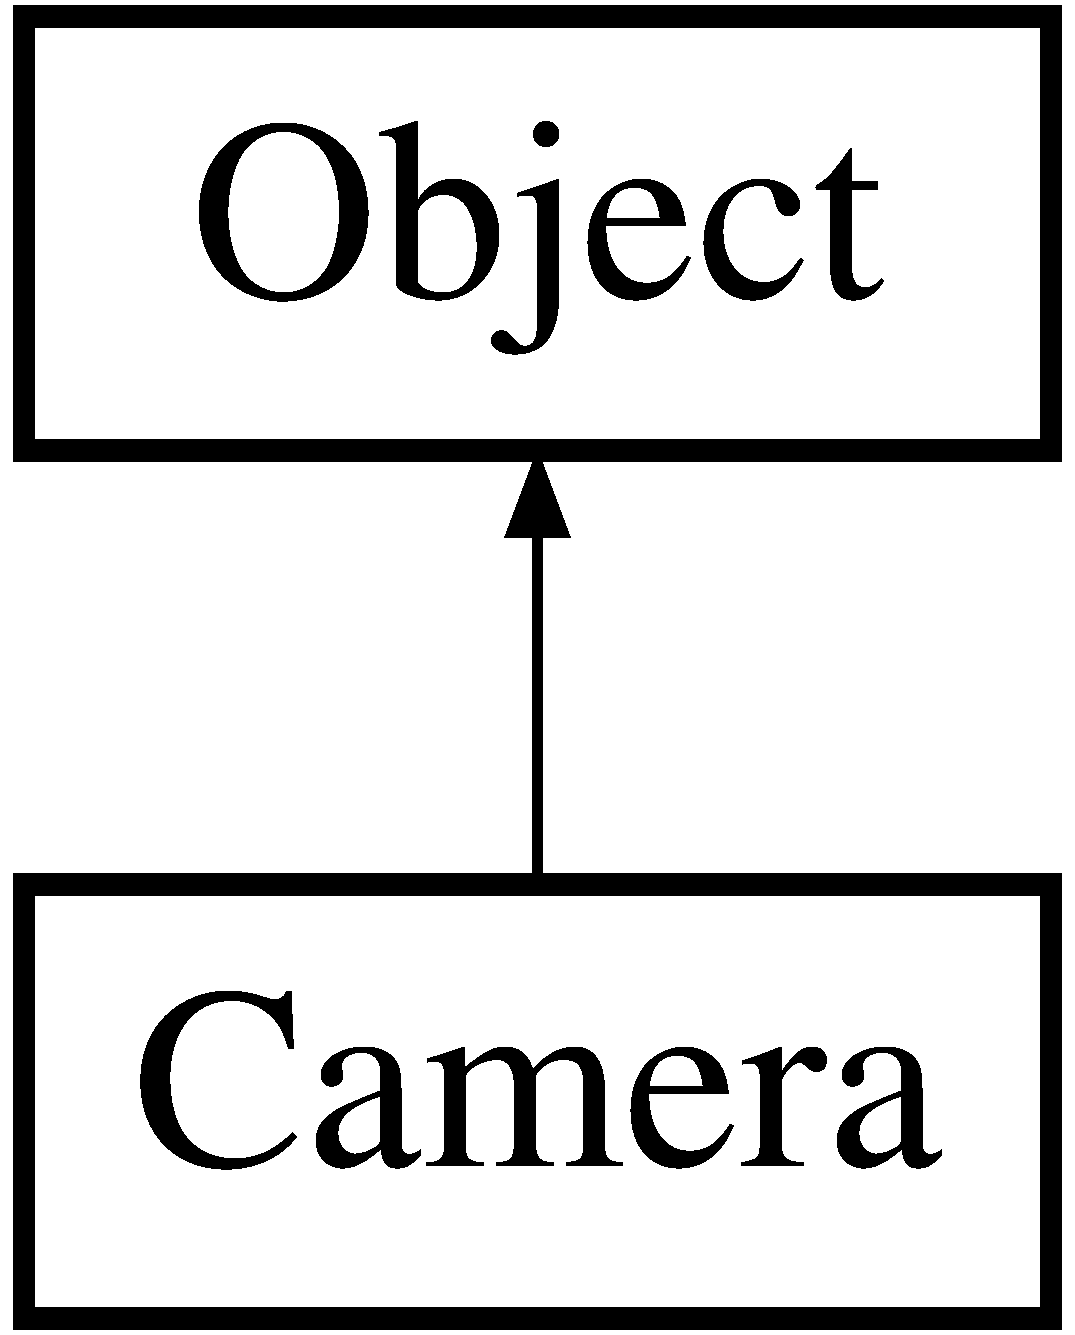
\includegraphics[height=2.000000cm]{class_object}
\end{center}
\end{figure}
\subsection*{Public Member Functions}
\begin{DoxyCompactItemize}
\item 
\mbox{\Hypertarget{class_object_a40860402e64d8008fb42329df7097cdb}\label{class_object_a40860402e64d8008fb42329df7097cdb}} 
\hyperlink{class_object_a40860402e64d8008fb42329df7097cdb}{Object} ()
\begin{DoxyCompactList}\small\item\em Default constructor. \end{DoxyCompactList}\item 
\mbox{\Hypertarget{class_object_ae8f5483f459e46687bd01e6f9977afd3}\label{class_object_ae8f5483f459e46687bd01e6f9977afd3}} 
\hyperlink{class_object_ae8f5483f459e46687bd01e6f9977afd3}{$\sim$\+Object} ()
\begin{DoxyCompactList}\small\item\em Default destructor. \end{DoxyCompactList}\item 
void \hyperlink{class_object_ab37a94ec1146c22546445d4baaf55697}{Init\+Object} (char $\ast$name, \hyperlink{class_object}{Object} $\ast$parent, \hyperlink{class_mesh}{Mesh} $\ast$mesh)
\begin{DoxyCompactList}\small\item\em Initialize object. \end{DoxyCompactList}\item 
void \hyperlink{class_object_a344ba3716db86c373345265935280968}{Set\+Parent} (\hyperlink{class_object}{Object} $\ast$parent)
\begin{DoxyCompactList}\small\item\em Set parent. \end{DoxyCompactList}\item 
\hyperlink{class_object}{Object} $\ast$ \hyperlink{class_object_a6f86d9e3b77d79cc3a6a4d57a5c9ed72}{Get\+Parent} ()
\begin{DoxyCompactList}\small\item\em Get parent. \end{DoxyCompactList}\item 
void \hyperlink{class_object_a6be7369b2a3382f82ea8d3e61c061b59}{Set\+Mesh} (\hyperlink{class_mesh}{Mesh} $\ast$mesh)
\begin{DoxyCompactList}\small\item\em Set mesh. \end{DoxyCompactList}\item 
\hyperlink{class_mesh}{Mesh} $\ast$ \hyperlink{class_object_ac59efbef5ea2a39576d7a057eb5e11ac}{Get\+Mesh} ()
\begin{DoxyCompactList}\small\item\em Get mesh. \end{DoxyCompactList}\item 
glm\+::mat4 $\ast$ \hyperlink{class_object_a58e26d2cc568b514884336ed279dc00c}{Get\+Model\+Matrix} ()
\begin{DoxyCompactList}\small\item\em Get model matrix. \end{DoxyCompactList}\item 
virtual void \hyperlink{class_object_a03bd9ae689e9535934f46222644f44aa}{Update} (float dt)
\begin{DoxyCompactList}\small\item\em Update object. \end{DoxyCompactList}\item 
void \hyperlink{class_object_adbffb47c9daf536f5ccd668d060a0490}{Set\+Position} (glm\+::vec3 position)
\begin{DoxyCompactList}\small\item\em Set object position. \end{DoxyCompactList}\item 
void \hyperlink{class_object_a08faf59cf967fae31dd3ed0aea43a372}{Set\+Scale} (glm\+::vec3 scale)
\begin{DoxyCompactList}\small\item\em Set object scale. \end{DoxyCompactList}\item 
void \hyperlink{class_object_a0aaf9cce0a37d5bb0af6eb11ab8dce64}{Set\+Euler\+Rotation} (glm\+::vec3 euler\+Angles)
\begin{DoxyCompactList}\small\item\em Set object rotaion. \end{DoxyCompactList}\item 
void \hyperlink{class_object_a5930b30196790ae109835e4f24a85b29}{Use\+Alternative\+Model\+Mat} (bool use)
\begin{DoxyCompactList}\small\item\em Use alternative model matrix. \end{DoxyCompactList}\item 
void \hyperlink{class_object_a178b374670d4681c61556a352276f96a}{Set\+Alternative\+Model\+Mat} (glm\+::mat4 model\+Mat)
\begin{DoxyCompactList}\small\item\em Set alternative model matrix. \end{DoxyCompactList}\item 
bool \hyperlink{class_object_ab1946453ecbf12a897ba6a363704cd86}{Set\+Active} (bool active)
\begin{DoxyCompactList}\small\item\em Set active object. \end{DoxyCompactList}\item 
bool \hyperlink{class_object_a49327b515f7e613c882f33c2b058ab98}{Is\+Active} ()
\begin{DoxyCompactList}\small\item\em Is active object. \end{DoxyCompactList}\end{DoxyCompactItemize}
\subsection*{Protected Member Functions}
\begin{DoxyCompactItemize}
\item 
void \hyperlink{class_object_af08c7cf7a01b230d6967551c52bdff63}{Update\+Matrix} ()
\begin{DoxyCompactList}\small\item\em Update model matrix. \end{DoxyCompactList}\end{DoxyCompactItemize}
\subsection*{Protected Attributes}
\begin{DoxyCompactItemize}
\item 
\mbox{\Hypertarget{class_object_ab37ae04046c449f0a8ab2833cfee5353}\label{class_object_ab37ae04046c449f0a8ab2833cfee5353}} 
char $\ast$ \hyperlink{class_object_ab37ae04046c449f0a8ab2833cfee5353}{m\+\_\+name}
\begin{DoxyCompactList}\small\item\em Name of the object. \end{DoxyCompactList}\item 
\mbox{\Hypertarget{class_object_a2ee3d966f96dbabae641ad390d82a6f3}\label{class_object_a2ee3d966f96dbabae641ad390d82a6f3}} 
\hyperlink{class_object}{Object} $\ast$ {\bfseries m\+\_\+parent}
\item 
\mbox{\Hypertarget{class_object_a82441da4d382a765bcf9c0a929f0a240}\label{class_object_a82441da4d382a765bcf9c0a929f0a240}} 
\hyperlink{class_mesh}{Mesh} $\ast$ \hyperlink{class_object_a82441da4d382a765bcf9c0a929f0a240}{m\+\_\+linked\+Mesh}
\begin{DoxyCompactList}\small\item\em \hyperlink{class_mesh}{Mesh} used by the object. \end{DoxyCompactList}\item 
\mbox{\Hypertarget{class_object_a9f5194b69d79120761526865270df0a6}\label{class_object_a9f5194b69d79120761526865270df0a6}} 
bool \hyperlink{class_object_a9f5194b69d79120761526865270df0a6}{m\+\_\+active}
\begin{DoxyCompactList}\small\item\em If the object is active or not for the updates. \end{DoxyCompactList}\item 
\mbox{\Hypertarget{class_object_a6628ff13c375c8a2bc9cc36c8585943c}\label{class_object_a6628ff13c375c8a2bc9cc36c8585943c}} 
glm\+::vec3 \hyperlink{class_object_a6628ff13c375c8a2bc9cc36c8585943c}{m\+\_\+global\+Position}
\begin{DoxyCompactList}\small\item\em Global position of the object. \end{DoxyCompactList}\item 
\mbox{\Hypertarget{class_object_ad717cc77240082806b13cd67338a4923}\label{class_object_ad717cc77240082806b13cd67338a4923}} 
glm\+::vec3 \hyperlink{class_object_ad717cc77240082806b13cd67338a4923}{m\+\_\+global\+Scale}
\begin{DoxyCompactList}\small\item\em Scale of the object. \end{DoxyCompactList}\item 
\mbox{\Hypertarget{class_object_a2b740c7fb22122a34286e0181fc69c8a}\label{class_object_a2b740c7fb22122a34286e0181fc69c8a}} 
glm\+::vec3 \hyperlink{class_object_a2b740c7fb22122a34286e0181fc69c8a}{m\+\_\+euler\+Angles}
\begin{DoxyCompactList}\small\item\em Rotation of the object in euler angles. \end{DoxyCompactList}\item 
\mbox{\Hypertarget{class_object_a63576ab555502bfb8de52e0f75b0d012}\label{class_object_a63576ab555502bfb8de52e0f75b0d012}} 
glm\+::mat4 \hyperlink{class_object_a63576ab555502bfb8de52e0f75b0d012}{m\+\_\+model\+Mat}
\begin{DoxyCompactList}\small\item\em Model matrix of the object. \end{DoxyCompactList}\item 
\mbox{\Hypertarget{class_object_aa8ca8a51906713190326b0b2667d975e}\label{class_object_aa8ca8a51906713190326b0b2667d975e}} 
glm\+::mat4 \hyperlink{class_object_aa8ca8a51906713190326b0b2667d975e}{m\+\_\+alt\+Model\+Mat}
\begin{DoxyCompactList}\small\item\em Alternative model matrix for more complex transformations. \end{DoxyCompactList}\item 
bool \hyperlink{class_object_ac7370557bcc44f3054712733de22d9ee}{m\+\_\+use\+Alt\+Mat} = false
\begin{DoxyCompactList}\small\item\em Use the default or the alternative model matrix. \end{DoxyCompactList}\item 
\mbox{\Hypertarget{class_object_a4e7183f8631f7473e648138facdee129}\label{class_object_a4e7183f8631f7473e648138facdee129}} 
bool \hyperlink{class_object_a4e7183f8631f7473e648138facdee129}{m\+\_\+update\+Matrix} = false
\begin{DoxyCompactList}\small\item\em Update the matrix if necessary. \end{DoxyCompactList}\end{DoxyCompactItemize}


\subsection{Detailed Description}
\hyperlink{class_object}{Object} class. 

The scene contains objects, which can have a mesh to display and execute logic. 

\subsection{Member Function Documentation}
\mbox{\Hypertarget{class_object_ac59efbef5ea2a39576d7a057eb5e11ac}\label{class_object_ac59efbef5ea2a39576d7a057eb5e11ac}} 
\index{Object@{Object}!Get\+Mesh@{Get\+Mesh}}
\index{Get\+Mesh@{Get\+Mesh}!Object@{Object}}
\subsubsection{\texorpdfstring{Get\+Mesh()}{GetMesh()}}
{\footnotesize\ttfamily \hyperlink{class_mesh}{Mesh} $\ast$ Object\+::\+Get\+Mesh (\begin{DoxyParamCaption}{ }\end{DoxyParamCaption})}



Get mesh. 

\begin{DoxyReturn}{Returns}
Linked mesh to the object. 
\end{DoxyReturn}
\mbox{\Hypertarget{class_object_a58e26d2cc568b514884336ed279dc00c}\label{class_object_a58e26d2cc568b514884336ed279dc00c}} 
\index{Object@{Object}!Get\+Model\+Matrix@{Get\+Model\+Matrix}}
\index{Get\+Model\+Matrix@{Get\+Model\+Matrix}!Object@{Object}}
\subsubsection{\texorpdfstring{Get\+Model\+Matrix()}{GetModelMatrix()}}
{\footnotesize\ttfamily glm\+::mat4 $\ast$ Object\+::\+Get\+Model\+Matrix (\begin{DoxyParamCaption}{ }\end{DoxyParamCaption})}



Get model matrix. 

\begin{DoxyReturn}{Returns}
Model matrix in use (default/standard). 
\end{DoxyReturn}
\mbox{\Hypertarget{class_object_a6f86d9e3b77d79cc3a6a4d57a5c9ed72}\label{class_object_a6f86d9e3b77d79cc3a6a4d57a5c9ed72}} 
\index{Object@{Object}!Get\+Parent@{Get\+Parent}}
\index{Get\+Parent@{Get\+Parent}!Object@{Object}}
\subsubsection{\texorpdfstring{Get\+Parent()}{GetParent()}}
{\footnotesize\ttfamily \hyperlink{class_object}{Object} $\ast$ Object\+::\+Get\+Parent (\begin{DoxyParamCaption}{ }\end{DoxyParamCaption})}



Get parent. 

\begin{DoxyReturn}{Returns}
Linked parent to the object. 
\end{DoxyReturn}
\mbox{\Hypertarget{class_object_ab37a94ec1146c22546445d4baaf55697}\label{class_object_ab37a94ec1146c22546445d4baaf55697}} 
\index{Object@{Object}!Init\+Object@{Init\+Object}}
\index{Init\+Object@{Init\+Object}!Object@{Object}}
\subsubsection{\texorpdfstring{Init\+Object()}{InitObject()}}
{\footnotesize\ttfamily void Object\+::\+Init\+Object (\begin{DoxyParamCaption}\item[{char $\ast$}]{name,  }\item[{\hyperlink{class_object}{Object} $\ast$}]{parent = {\ttfamily nullptr},  }\item[{\hyperlink{class_mesh}{Mesh} $\ast$}]{mesh = {\ttfamily nullptr} }\end{DoxyParamCaption})}



Initialize object. 


\begin{DoxyParams}{Parameters}
{\em name} & Name of the object. \\
\hline
{\em parent} & Parent of the object. \\
\hline
{\em mesh} & \hyperlink{class_mesh}{Mesh} of the object. \\
\hline
\end{DoxyParams}
\mbox{\Hypertarget{class_object_a49327b515f7e613c882f33c2b058ab98}\label{class_object_a49327b515f7e613c882f33c2b058ab98}} 
\index{Object@{Object}!Is\+Active@{Is\+Active}}
\index{Is\+Active@{Is\+Active}!Object@{Object}}
\subsubsection{\texorpdfstring{Is\+Active()}{IsActive()}}
{\footnotesize\ttfamily bool Object\+::\+Is\+Active (\begin{DoxyParamCaption}{ }\end{DoxyParamCaption})}



Is active object. 

\begin{DoxyReturn}{Returns}
If the object is active or not. 
\end{DoxyReturn}
\mbox{\Hypertarget{class_object_ab1946453ecbf12a897ba6a363704cd86}\label{class_object_ab1946453ecbf12a897ba6a363704cd86}} 
\index{Object@{Object}!Set\+Active@{Set\+Active}}
\index{Set\+Active@{Set\+Active}!Object@{Object}}
\subsubsection{\texorpdfstring{Set\+Active()}{SetActive()}}
{\footnotesize\ttfamily bool Object\+::\+Set\+Active (\begin{DoxyParamCaption}\item[{bool}]{active }\end{DoxyParamCaption})}



Set active object. 

Activates or deactivates the object. 
\begin{DoxyParams}{Parameters}
{\em active} & Sets the object active or not. \\
\hline
\end{DoxyParams}
\begin{DoxyReturn}{Returns}
If the object is active or not. 
\end{DoxyReturn}
\mbox{\Hypertarget{class_object_a178b374670d4681c61556a352276f96a}\label{class_object_a178b374670d4681c61556a352276f96a}} 
\index{Object@{Object}!Set\+Alternative\+Model\+Mat@{Set\+Alternative\+Model\+Mat}}
\index{Set\+Alternative\+Model\+Mat@{Set\+Alternative\+Model\+Mat}!Object@{Object}}
\subsubsection{\texorpdfstring{Set\+Alternative\+Model\+Mat()}{SetAlternativeModelMat()}}
{\footnotesize\ttfamily void Object\+::\+Set\+Alternative\+Model\+Mat (\begin{DoxyParamCaption}\item[{glm\+::mat4}]{model\+Mat }\end{DoxyParamCaption})}



Set alternative model matrix. 


\begin{DoxyParams}{Parameters}
{\em model\+Mat} & Sets the alternative model matrix of the object \\
\hline
\end{DoxyParams}
\mbox{\Hypertarget{class_object_a0aaf9cce0a37d5bb0af6eb11ab8dce64}\label{class_object_a0aaf9cce0a37d5bb0af6eb11ab8dce64}} 
\index{Object@{Object}!Set\+Euler\+Rotation@{Set\+Euler\+Rotation}}
\index{Set\+Euler\+Rotation@{Set\+Euler\+Rotation}!Object@{Object}}
\subsubsection{\texorpdfstring{Set\+Euler\+Rotation()}{SetEulerRotation()}}
{\footnotesize\ttfamily void Object\+::\+Set\+Euler\+Rotation (\begin{DoxyParamCaption}\item[{glm\+::vec3}]{euler\+Angles }\end{DoxyParamCaption})}



Set object rotaion. 

Rotates the object using euler angles. 
\begin{DoxyParams}{Parameters}
{\em euler\+Angles} & Rotation of the object. \\
\hline
\end{DoxyParams}
\mbox{\Hypertarget{class_object_a6be7369b2a3382f82ea8d3e61c061b59}\label{class_object_a6be7369b2a3382f82ea8d3e61c061b59}} 
\index{Object@{Object}!Set\+Mesh@{Set\+Mesh}}
\index{Set\+Mesh@{Set\+Mesh}!Object@{Object}}
\subsubsection{\texorpdfstring{Set\+Mesh()}{SetMesh()}}
{\footnotesize\ttfamily void Object\+::\+Set\+Mesh (\begin{DoxyParamCaption}\item[{\hyperlink{class_mesh}{Mesh} $\ast$}]{mesh }\end{DoxyParamCaption})}



Set mesh. 


\begin{DoxyParams}{Parameters}
{\em mesh} & Link mesh to the object. \\
\hline
\end{DoxyParams}
\mbox{\Hypertarget{class_object_a344ba3716db86c373345265935280968}\label{class_object_a344ba3716db86c373345265935280968}} 
\index{Object@{Object}!Set\+Parent@{Set\+Parent}}
\index{Set\+Parent@{Set\+Parent}!Object@{Object}}
\subsubsection{\texorpdfstring{Set\+Parent()}{SetParent()}}
{\footnotesize\ttfamily void Object\+::\+Set\+Parent (\begin{DoxyParamCaption}\item[{\hyperlink{class_object}{Object} $\ast$}]{parent }\end{DoxyParamCaption})}



Set parent. 


\begin{DoxyParams}{Parameters}
{\em parent} & Link parent to the object. \\
\hline
\end{DoxyParams}
\mbox{\Hypertarget{class_object_adbffb47c9daf536f5ccd668d060a0490}\label{class_object_adbffb47c9daf536f5ccd668d060a0490}} 
\index{Object@{Object}!Set\+Position@{Set\+Position}}
\index{Set\+Position@{Set\+Position}!Object@{Object}}
\subsubsection{\texorpdfstring{Set\+Position()}{SetPosition()}}
{\footnotesize\ttfamily void Object\+::\+Set\+Position (\begin{DoxyParamCaption}\item[{glm\+::vec3}]{position }\end{DoxyParamCaption})}



Set object position. 


\begin{DoxyParams}{Parameters}
{\em position} & Moves the object to a specified position in global space. \\
\hline
\end{DoxyParams}
\mbox{\Hypertarget{class_object_a08faf59cf967fae31dd3ed0aea43a372}\label{class_object_a08faf59cf967fae31dd3ed0aea43a372}} 
\index{Object@{Object}!Set\+Scale@{Set\+Scale}}
\index{Set\+Scale@{Set\+Scale}!Object@{Object}}
\subsubsection{\texorpdfstring{Set\+Scale()}{SetScale()}}
{\footnotesize\ttfamily void Object\+::\+Set\+Scale (\begin{DoxyParamCaption}\item[{glm\+::vec3}]{scale }\end{DoxyParamCaption})}



Set object scale. 


\begin{DoxyParams}{Parameters}
{\em scale} & Scales the object. \\
\hline
\end{DoxyParams}
\mbox{\Hypertarget{class_object_a03bd9ae689e9535934f46222644f44aa}\label{class_object_a03bd9ae689e9535934f46222644f44aa}} 
\index{Object@{Object}!Update@{Update}}
\index{Update@{Update}!Object@{Object}}
\subsubsection{\texorpdfstring{Update()}{Update()}}
{\footnotesize\ttfamily void Object\+::\+Update (\begin{DoxyParamCaption}\item[{float}]{dt }\end{DoxyParamCaption})\hspace{0.3cm}{\ttfamily [virtual]}}



Update object. 

Logic used for the object. 
\begin{DoxyParams}{Parameters}
{\em dt} & Delta time. \\
\hline
\end{DoxyParams}
\mbox{\Hypertarget{class_object_af08c7cf7a01b230d6967551c52bdff63}\label{class_object_af08c7cf7a01b230d6967551c52bdff63}} 
\index{Object@{Object}!Update\+Matrix@{Update\+Matrix}}
\index{Update\+Matrix@{Update\+Matrix}!Object@{Object}}
\subsubsection{\texorpdfstring{Update\+Matrix()}{UpdateMatrix()}}
{\footnotesize\ttfamily void Object\+::\+Update\+Matrix (\begin{DoxyParamCaption}{ }\end{DoxyParamCaption})\hspace{0.3cm}{\ttfamily [protected]}}



Update model matrix. 

Updates the model matrix if necessary. \mbox{\Hypertarget{class_object_a5930b30196790ae109835e4f24a85b29}\label{class_object_a5930b30196790ae109835e4f24a85b29}} 
\index{Object@{Object}!Use\+Alternative\+Model\+Mat@{Use\+Alternative\+Model\+Mat}}
\index{Use\+Alternative\+Model\+Mat@{Use\+Alternative\+Model\+Mat}!Object@{Object}}
\subsubsection{\texorpdfstring{Use\+Alternative\+Model\+Mat()}{UseAlternativeModelMat()}}
{\footnotesize\ttfamily void Object\+::\+Use\+Alternative\+Model\+Mat (\begin{DoxyParamCaption}\item[{bool}]{use }\end{DoxyParamCaption})}



Use alternative model matrix. 


\begin{DoxyParams}{Parameters}
{\em use} & True\+: use the alternative model matrix. False\+: use the default model matrix. \\
\hline
\end{DoxyParams}


\subsection{Member Data Documentation}
\mbox{\Hypertarget{class_object_ac7370557bcc44f3054712733de22d9ee}\label{class_object_ac7370557bcc44f3054712733de22d9ee}} 
\index{Object@{Object}!m\+\_\+use\+Alt\+Mat@{m\+\_\+use\+Alt\+Mat}}
\index{m\+\_\+use\+Alt\+Mat@{m\+\_\+use\+Alt\+Mat}!Object@{Object}}
\subsubsection{\texorpdfstring{m\+\_\+use\+Alt\+Mat}{m\_useAltMat}}
{\footnotesize\ttfamily bool Object\+::m\+\_\+use\+Alt\+Mat = false\hspace{0.3cm}{\ttfamily [protected]}}



Use the default or the alternative model matrix. 

\begin{DoxySeeAlso}{See also}
\hyperlink{class_object_a63576ab555502bfb8de52e0f75b0d012}{m\+\_\+model\+Mat} 

\hyperlink{class_object_aa8ca8a51906713190326b0b2667d975e}{m\+\_\+alt\+Model\+Mat} 
\end{DoxySeeAlso}


The documentation for this class was generated from the following files\+:\begin{DoxyCompactItemize}
\item 
Object.\+h\item 
Object.\+cpp\end{DoxyCompactItemize}

\hypertarget{class_point_light}{}\section{Point\+Light Class Reference}
\label{class_point_light}\index{Point\+Light@{Point\+Light}}


\hyperlink{class_point_light}{Point\+Light} class.  




{\ttfamily \#include $<$Point\+Light.\+h$>$}

Inheritance diagram for Point\+Light\+:\begin{figure}[H]
\begin{center}
\leavevmode
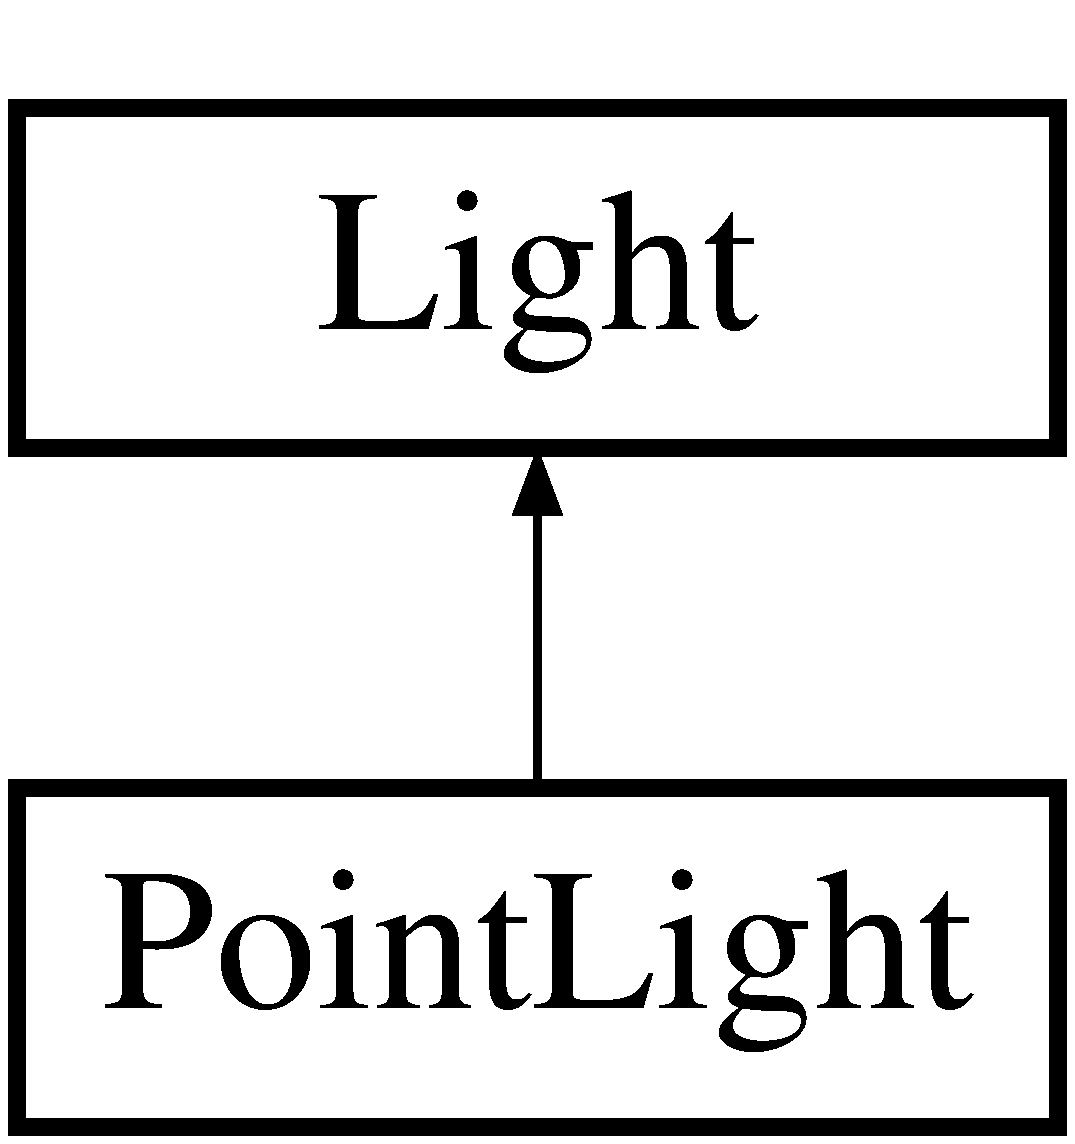
\includegraphics[height=2.000000cm]{class_point_light}
\end{center}
\end{figure}
\subsection*{Public Member Functions}
\begin{DoxyCompactItemize}
\item 
\hyperlink{class_point_light_abbfdf5f05b559c49016f8bb97b0ca414}{Point\+Light} ()
\begin{DoxyCompactList}\small\item\em Class constructor. \end{DoxyCompactList}\item 
\hyperlink{class_point_light_aa12d9005d5372dbbe655a82231634341}{$\sim$\+Point\+Light} ()
\begin{DoxyCompactList}\small\item\em Class destructor. \end{DoxyCompactList}\item 
void \hyperlink{class_point_light_a54075ad125124b48c3ae0de94f8846ec}{Set\+Position} (glm\+::vec3 position)
\begin{DoxyCompactList}\small\item\em Position setter. \end{DoxyCompactList}\item 
void \hyperlink{class_point_light_a5dee3d9dfd33530fd0b5c4e3caa733a5}{Set\+Attenuation} (glm\+::vec3 attenuation)
\begin{DoxyCompactList}\small\item\em Attenuation setter. \end{DoxyCompactList}\end{DoxyCompactItemize}
\subsection*{Additional Inherited Members}


\subsection{Detailed Description}
\hyperlink{class_point_light}{Point\+Light} class. 

Class used to define a point light. 

\subsection{Constructor \& Destructor Documentation}
\mbox{\Hypertarget{class_point_light_abbfdf5f05b559c49016f8bb97b0ca414}\label{class_point_light_abbfdf5f05b559c49016f8bb97b0ca414}} 
\index{Point\+Light@{Point\+Light}!Point\+Light@{Point\+Light}}
\index{Point\+Light@{Point\+Light}!Point\+Light@{Point\+Light}}
\subsubsection{\texorpdfstring{Point\+Light()}{PointLight()}}
{\footnotesize\ttfamily Point\+Light\+::\+Point\+Light (\begin{DoxyParamCaption}{ }\end{DoxyParamCaption})}



Class constructor. 

\hyperlink{class_point_light}{Point\+Light} class constructor. \mbox{\Hypertarget{class_point_light_aa12d9005d5372dbbe655a82231634341}\label{class_point_light_aa12d9005d5372dbbe655a82231634341}} 
\index{Point\+Light@{Point\+Light}!````~Point\+Light@{$\sim$\+Point\+Light}}
\index{````~Point\+Light@{$\sim$\+Point\+Light}!Point\+Light@{Point\+Light}}
\subsubsection{\texorpdfstring{$\sim$\+Point\+Light()}{~PointLight()}}
{\footnotesize\ttfamily Point\+Light\+::$\sim$\+Point\+Light (\begin{DoxyParamCaption}{ }\end{DoxyParamCaption})}



Class destructor. 

Poijnt\+Light class destructor. 

\subsection{Member Function Documentation}
\mbox{\Hypertarget{class_point_light_a5dee3d9dfd33530fd0b5c4e3caa733a5}\label{class_point_light_a5dee3d9dfd33530fd0b5c4e3caa733a5}} 
\index{Point\+Light@{Point\+Light}!Set\+Attenuation@{Set\+Attenuation}}
\index{Set\+Attenuation@{Set\+Attenuation}!Point\+Light@{Point\+Light}}
\subsubsection{\texorpdfstring{Set\+Attenuation()}{SetAttenuation()}}
{\footnotesize\ttfamily void Point\+Light\+::\+Set\+Attenuation (\begin{DoxyParamCaption}\item[{glm\+::vec3}]{attenuation }\end{DoxyParamCaption})}



Attenuation setter. 


\begin{DoxyParams}{Parameters}
{\em attenuation} & 3D vector to set as new attenuation. \\
\hline
\end{DoxyParams}
\mbox{\Hypertarget{class_point_light_a54075ad125124b48c3ae0de94f8846ec}\label{class_point_light_a54075ad125124b48c3ae0de94f8846ec}} 
\index{Point\+Light@{Point\+Light}!Set\+Position@{Set\+Position}}
\index{Set\+Position@{Set\+Position}!Point\+Light@{Point\+Light}}
\subsubsection{\texorpdfstring{Set\+Position()}{SetPosition()}}
{\footnotesize\ttfamily void Point\+Light\+::\+Set\+Position (\begin{DoxyParamCaption}\item[{glm\+::vec3}]{position }\end{DoxyParamCaption})}



Position setter. 


\begin{DoxyParams}{Parameters}
{\em position} & 3D vector to set as new postion. \\
\hline
\end{DoxyParams}


The documentation for this class was generated from the following files\+:\begin{DoxyCompactItemize}
\item 
Point\+Light.\+h\item 
Point\+Light.\+cpp\end{DoxyCompactItemize}

\hypertarget{class_scene}{}\section{Scene Class Reference}
\label{class_scene}\index{Scene@{Scene}}
\subsection*{Public Member Functions}
\begin{DoxyCompactItemize}
\item 
\mbox{\Hypertarget{class_scene_a71708279f69885e838e288c6689ddd1c}\label{class_scene_a71708279f69885e838e288c6689ddd1c}} 
void {\bfseries Render\+Loop} ()
\item 
\mbox{\Hypertarget{class_scene_ab0293e9c900f18ce4ca26621d4b7ddfe}\label{class_scene_ab0293e9c900f18ce4ca26621d4b7ddfe}} 
void {\bfseries Update\+Loop} ()
\item 
\mbox{\Hypertarget{class_scene_a6f0f7af3d07acbee2d6864c3ded98351}\label{class_scene_a6f0f7af3d07acbee2d6864c3ded98351}} 
\hyperlink{class_shader}{Shader} $\ast$ {\bfseries Load\+Shader} (char $\ast$vertex\+Shader, char $\ast$fragment\+Shader)
\item 
\mbox{\Hypertarget{class_scene_a660e1d1c0aebaff994ea6d36d1e9fec5}\label{class_scene_a660e1d1c0aebaff994ea6d36d1e9fec5}} 
\hyperlink{class_mesh}{Mesh} $\ast$ {\bfseries Load\+Mesh} (char $\ast$mesh, \hyperlink{class_shader}{Shader} $\ast$shader)
\item 
\mbox{\Hypertarget{class_scene_a676cf764adad1d7e30311582ccae2b7e}\label{class_scene_a676cf764adad1d7e30311582ccae2b7e}} 
\hyperlink{class_mesh}{Mesh} $\ast$ {\bfseries Load\+Mesh} (\hyperlink{class_mesh}{Mesh} $\ast$mesh, \hyperlink{class_shader}{Shader} $\ast$shader)
\item 
\mbox{\Hypertarget{class_scene_adfdea29bf0ed9107c28f99fb8ebe34d1}\label{class_scene_adfdea29bf0ed9107c28f99fb8ebe34d1}} 
\hyperlink{class_object}{Object} $\ast$ {\bfseries Create\+Object} (\hyperlink{class_mesh}{Mesh} $\ast$mesh, char $\ast$name)
\item 
\mbox{\Hypertarget{class_scene_a8ba56754e230d7a99736c5232bd912ea}\label{class_scene_a8ba56754e230d7a99736c5232bd912ea}} 
\hyperlink{class_directional_light}{Directional\+Light} $\ast$ {\bfseries Add\+Directional\+Light} ()
\item 
\mbox{\Hypertarget{class_scene_ac33b9cc536096a447892f524802dd2ec}\label{class_scene_ac33b9cc536096a447892f524802dd2ec}} 
\hyperlink{class_point_light}{Point\+Light} $\ast$ {\bfseries Add\+Point\+Light} ()
\item 
\mbox{\Hypertarget{class_scene_a5086a9e37b94c2dfb30dfacbee668c79}\label{class_scene_a5086a9e37b94c2dfb30dfacbee668c79}} 
\hyperlink{class_spot_light}{Spot\+Light} $\ast$ {\bfseries Add\+Spot\+Light} ()
\end{DoxyCompactItemize}
\subsection*{Public Attributes}
\begin{DoxyCompactItemize}
\item 
\mbox{\Hypertarget{class_scene_afed13ec4ba2d7ab75b273d507911b498}\label{class_scene_afed13ec4ba2d7ab75b273d507911b498}} 
\hyperlink{class_camera}{Camera} {\bfseries camera}
\item 
\mbox{\Hypertarget{class_scene_a5f692c13f2db4299793ffc4d36c7e2ba}\label{class_scene_a5f692c13f2db4299793ffc4d36c7e2ba}} 
std\+::vector$<$ \hyperlink{class_shader}{Shader} $>$ {\bfseries scene\+Shaders}
\item 
\mbox{\Hypertarget{class_scene_a7be2dbccfae00f70b1d07b2c4d738ece}\label{class_scene_a7be2dbccfae00f70b1d07b2c4d738ece}} 
std\+::vector$<$ \hyperlink{class_mesh}{Mesh} $>$ {\bfseries scene\+Meshes}
\item 
\mbox{\Hypertarget{class_scene_ad9e4d19ec059a134617ee31d1df03714}\label{class_scene_ad9e4d19ec059a134617ee31d1df03714}} 
std\+::vector$<$ \hyperlink{class_object}{Object} $>$ {\bfseries scene\+Objects}
\item 
\mbox{\Hypertarget{class_scene_aa98be8079c5bed3a6a24aa55fe15f3f0}\label{class_scene_aa98be8079c5bed3a6a24aa55fe15f3f0}} 
std\+::list$<$ \hyperlink{class_light}{Light} $>$ {\bfseries scene\+Lights}
\item 
\mbox{\Hypertarget{class_scene_a4624158c6d315465401ccdda659bc13b}\label{class_scene_a4624158c6d315465401ccdda659bc13b}} 
float {\bfseries delta\+Time}
\end{DoxyCompactItemize}


The documentation for this class was generated from the following files\+:\begin{DoxyCompactItemize}
\item 
Scene.\+h\item 
Scene.\+cpp\end{DoxyCompactItemize}

\hypertarget{class_shader}{}\section{Shader Class Reference}
\label{class_shader}\index{Shader@{Shader}}
\subsection*{Public Member Functions}
\begin{DoxyCompactItemize}
\item 
\hypertarget{class_shader_a7e02f1eaec796a7fc02c3191ce9fa5d4}{}{\bfseries Shader} (const char $\ast$vertex, const char $\ast$fragment)\label{class_shader_a7e02f1eaec796a7fc02c3191ce9fa5d4}

\item 
\hypertarget{class_shader_a4bb445563c154a27e3dc0e1036690841}{}void {\bfseries render} (std\+::list$<$ \hyperlink{class_light}{Light} $>$ \&light\+V, \hyperlink{class_camera}{Camera} \&camera)\label{class_shader_a4bb445563c154a27e3dc0e1036690841}

\item 
\hypertarget{class_shader_ab6af37727a2f0a0e5f31fb05e9137853}{}void {\bfseries add\+Mesh} (\hyperlink{class_mesh}{Mesh} $\ast$mesh)\label{class_shader_ab6af37727a2f0a0e5f31fb05e9137853}

\item 
\hypertarget{class_shader_ad52dea081c158e54bd3dcd5168623a3f}{}int {\bfseries get\+In\+Pos} ()\label{class_shader_ad52dea081c158e54bd3dcd5168623a3f}

\item 
\hypertarget{class_shader_ae39ec6d01ef565e170cce67c75d3fa3d}{}int {\bfseries get\+In\+Color} ()\label{class_shader_ae39ec6d01ef565e170cce67c75d3fa3d}

\item 
\hypertarget{class_shader_a9647f6a0356188f9f56787dbebde4731}{}int {\bfseries get\+In\+Normal} ()\label{class_shader_a9647f6a0356188f9f56787dbebde4731}

\item 
\hypertarget{class_shader_a386214ac36c08a8405ec458f75d17d12}{}int {\bfseries get\+In\+Tex\+Coord} ()\label{class_shader_a386214ac36c08a8405ec458f75d17d12}

\item 
\hypertarget{class_shader_aad0dc2b502af0bcf6c5aa99e60fc296a}{}int {\bfseries get\+In\+Tangent} ()\label{class_shader_aad0dc2b502af0bcf6c5aa99e60fc296a}

\end{DoxyCompactItemize}


The documentation for this class was generated from the following files\+:\begin{DoxyCompactItemize}
\item 
Shader.\+h\item 
Shader.\+cpp\end{DoxyCompactItemize}

\hypertarget{class_spot_light}{}\section{Spot\+Light Class Reference}
\label{class_spot_light}\index{Spot\+Light@{Spot\+Light}}
Inheritance diagram for Spot\+Light\+:\begin{figure}[H]
\begin{center}
\leavevmode
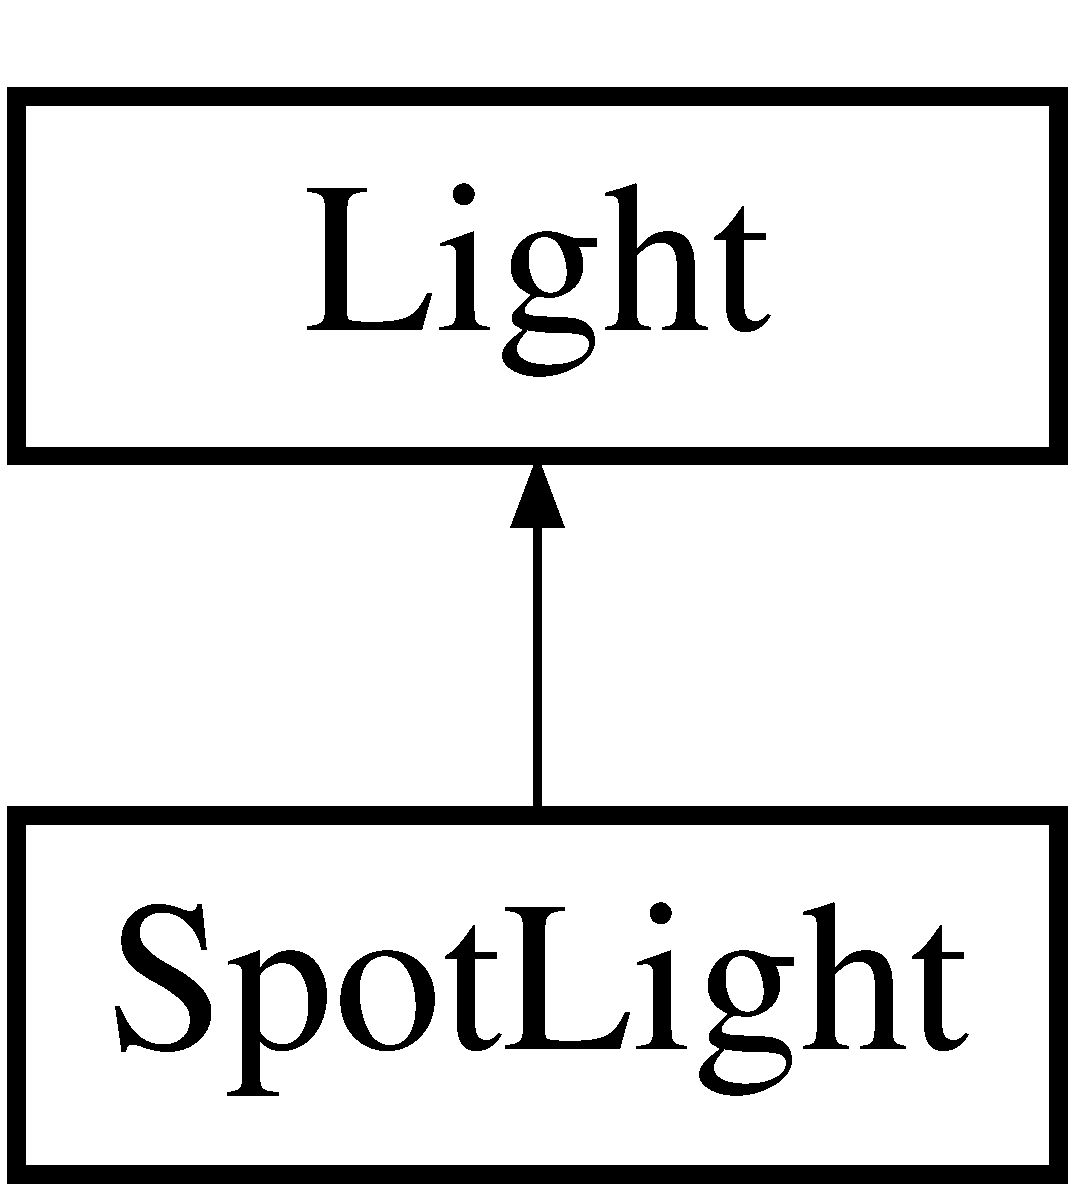
\includegraphics[height=2.000000cm]{class_spot_light}
\end{center}
\end{figure}
\subsection*{Public Member Functions}
\begin{DoxyCompactItemize}
\item 
\hypertarget{class_spot_light_a66a62acf516440ac717b4aa464c3c94a}{}void {\bfseries Set\+Position} (glm\+::vec3 position)\label{class_spot_light_a66a62acf516440ac717b4aa464c3c94a}

\item 
\hypertarget{class_spot_light_ac8239339ffa7dd31ea07a4cdcc36c4f4}{}void {\bfseries Set\+Direction} (glm\+::vec3 direction)\label{class_spot_light_ac8239339ffa7dd31ea07a4cdcc36c4f4}

\item 
\hypertarget{class_spot_light_addcb3fc1007d25b33f4275ff16f26073}{}void {\bfseries Set\+Attenuation} (glm\+::vec3 attenuation)\label{class_spot_light_addcb3fc1007d25b33f4275ff16f26073}

\item 
\hypertarget{class_spot_light_ac7a4c2343ed2d8da4f2511d50318cb5f}{}void {\bfseries Set\+Cos\+Cut\+Off} (G\+Lfloat cos\+Cut\+Off)\label{class_spot_light_ac7a4c2343ed2d8da4f2511d50318cb5f}

\item 
\hypertarget{class_spot_light_aa45ba8d849a2a9a994f144c2610fa498}{}void {\bfseries Set\+Spot\+Exponent} (G\+Lfloat spot\+Exponent)\label{class_spot_light_aa45ba8d849a2a9a994f144c2610fa498}

\end{DoxyCompactItemize}
\subsection*{Additional Inherited Members}


The documentation for this class was generated from the following files\+:\begin{DoxyCompactItemize}
\item 
Spot\+Light.\+h\item 
Spot\+Light.\+cpp\end{DoxyCompactItemize}

%--- End generated contents ---

% Index
\backmatter
\newpage
\phantomsection
\clearemptydoublepage
\addcontentsline{toc}{chapter}{Index}
\printindex

\end{document}
